\chapter{Stokes 问题}\label{ch:9}
\SourcePage{307}

本章讨论 Stokes 微分方程组,可写成
\begin{equation}\tag{9.1}\label{eq:9.1}
  \begin{cases}
    a_0\boldsymbol{u}-\nu\Delta\boldsymbol{u}+\nabla p=\boldsymbol{f},
      &\text{在 }\Omega\subset\mathbb R^d\text{ 内},\quad d=2,3,\\
    \operatorname{div}\boldsymbol{u}=0,&\text{在 }\Omega\text{ 内},\\
    \boldsymbol{u}=0,&\text{在 }\partial\Omega\text{ 上},
  \end{cases}
\end{equation}
其中 \(a_0\ge0\) 和 \(\nu>0\) 是给定常数,\(\boldsymbol{f}\colon\Omega\to\mathbb R^d\) 是给定函数,\(\boldsymbol{u}\colon\Omega\to\mathbb R^d\) 和 \(p\colon\Omega\to\mathbb R\) 是待求的未知量.

在流体力学中求解局限于 \(\Omega\) 内的流动的 Navier--Stokes 方程时,\eqref{eq:9.1}可作为求解过程中的一环出现,例如用半隐式格式或分裂法推进时间时.在这些情形下,\(a_0\) 几乎总起时间步长倒数的作用.Navier--Stokes 方程的完整推导见第~\BookRef{sec:13.1}{13.1}~节.另一个例子是黏性很大、Reynolds 数很小的流体缓慢运动,此时 \(a_0=0\),而 \(\boldsymbol{f}\) 表示单位质量所受的外力.两种情形中,\(p\) 都表示流体压力与密度之比,\(\boldsymbol{u}\) 则表示速度.

\eqref{eq:9.1}采用经典的齐次 Dirichlet 边界条件.也可在 \(\partial\Omega\) 上施加涉及 \(\boldsymbol{u}\) 的法向导数,或该导数与 \(p\) 的线性组合的其他条件,这将在第~\BookRef{sec:10.1.1}{10.1.1}~节指出.

\section{数学表述与分析}\label{sec:9.1}

假定 \(\boldsymbol{f}\in(L^2(\Omega))^d\),并令
\(\mathcal V:=\{\boldsymbol{v}\in(\mathcal D(\Omega))^d\mid\operatorname{div}\boldsymbol{v}=0\}\)
及 \(V:=(H_0^1(\Omega))^d\),其中 \(V\) 为 Hilbert 空间.由\eqref{eq:9.1}的第一个方程以及 Green 公式\eqref{eq:5.1.2}和\eqref{eq:5.1.5},得到
\begin{equation}\label{eq:9.1.1}
  a_0(\boldsymbol{u},\boldsymbol{v})+\nu(\nabla\boldsymbol{u},\nabla\boldsymbol{v})
      -(p,\operatorname{div}\boldsymbol{v})=(\boldsymbol{f},\boldsymbol{v})
      \qquad\forall\,\boldsymbol{v}\in(\mathcal D(\Omega))^d,
\end{equation}
因而
\SourcePage{308}
\begin{equation}\label{eq:9.1.2}
  a_0(\boldsymbol{u},\boldsymbol{v})+\nu(\nabla\boldsymbol{u},\nabla\boldsymbol{v})
      =(\boldsymbol{f},\boldsymbol{v})\qquad\forall\,\boldsymbol{v}\in\mathcal V.
\end{equation}

\begin{definition*}
定义空间
\begin{equation}\label{eq:9.1.3}
  V_{\mathrm{div}}:=\{\boldsymbol{v}\in V\mid\operatorname{div}\boldsymbol{v}=0\}.
\end{equation}
\end{definition*}
这是 \(V\) 的闭子空间.由 Poincaré 不等式\eqref{eq:1.3.2}可知,它关于范数
\begin{equation}\label{eq:9.1.4}
  \|\boldsymbol{v}\|:=\|\nabla\boldsymbol{v}\|_0
\end{equation}
为 Hilbert 空间.由此可知,双线性形式
\begin{equation}\label{eq:9.1.5}
  a(\boldsymbol{w},\boldsymbol{v}):=a_0(\boldsymbol{w},\boldsymbol{v})
      +\nu(\nabla\boldsymbol{w},\nabla\boldsymbol{v}),\qquad \boldsymbol{w},\boldsymbol{v}\in V
\end{equation}
在 \(V_{\mathrm{div}}\times V_{\mathrm{div}}\) 上具有强制性.此外,映射 \(\boldsymbol{v}\mapsto(\boldsymbol{f},\boldsymbol{v})\) 在 \(V_{\mathrm{div}}\) 上线性且连续,所以由 Lax--Milgram 引理可知,问题
\begin{equation}\label{eq:9.1.6}
  \text{求 }\boldsymbol{u}\in V_{\mathrm{div}},\quad\text{使}\quad
     a(\boldsymbol{u},\boldsymbol{v})=(\boldsymbol{f},\boldsymbol{v})
      \qquad\forall\,\boldsymbol{v}\in V_{\mathrm{div}}
\end{equation}
有唯一解.

下面将用到下列结果.

\begin{lemma}[]{9.1.1}
设 \(\Omega\) 为 \(\mathbb R^d\) 中具有 Lipschitz 连续边界的有界区域,且 \(L\in V'\),即 \(L\) 是 \(V\) 上的连续线性泛函.则 \(L\) 在 \(V_{\mathrm{div}}\) 上恒为零,当且仅当存在 \(p\in L^2(\Omega)\),使
\begin{equation}\label{eq:9.1.7}
  L(\boldsymbol{v})=(p,\operatorname{div}\boldsymbol{v})\qquad\forall\,\boldsymbol{v}\in V.
\end{equation}
此外,\eqref{eq:9.1.7}确定的函数 \(p\) 在相差一个加性常数的意义下唯一.
\end{lemma}

为简便起见,这里省略这一引理的证明,例如可见\BookCite{girault-raviart1986}{Girault 和 Raviart(1986)}第 22 页.

现在可以证明下列定理.

\begin{theorem}[]{9.1.1}
设 \(\Omega\) 为 \(\mathbb R^d\) 中具有 Lipschitz 连续边界的有界区域.对于每个 \(\boldsymbol{f}\in(L^2(\Omega))^d\),令 \(\boldsymbol{u}\) 为\eqref{eq:9.1.6}的解.则存在 \(p\in L^2(\Omega)\),在相差一个加性常数的意义下唯一,使
\begin{equation}\label{eq:9.1.8}
  a(\boldsymbol{u},\boldsymbol{v})-(p,\operatorname{div}\boldsymbol{v})=(\boldsymbol{f},\boldsymbol{v})
      \qquad\forall\,\boldsymbol{v}\in V.
\end{equation}
\end{theorem}

\begin{proof}
令 \(\boldsymbol{u}\) 是\eqref{eq:9.1.6}的解,并定义
\[
  L(\boldsymbol{v}):=a(\boldsymbol{u},\boldsymbol{v})-(\boldsymbol{f},\boldsymbol{v})
      \qquad\forall\,\boldsymbol{v}\in V.
\]
\SourcePage{309}由\eqref{eq:9.1.6}可知,\(L\) 满足引理~\ref{lem:9.1.1}的假设.因此,存在 \(p\in L^2(\Omega)\),使 \((\boldsymbol{u},p)\) 是\eqref{eq:9.1.8}的解.\hfill\(\square\)
\end{proof}

现在给出另一种方法.定义 Hilbert 空间 \(Q=L_0^2(\Omega)\),其中
\begin{equation}\label{eq:9.1.9}
  L_0^2(\Omega):=\left\{q\in L^2(\Omega)\ \middle|\ \int_\Omega q=0\right\},
\end{equation}
并定义双线性形式
\begin{equation}\label{eq:9.1.10}
  b(\boldsymbol{v},q):=-(q,\operatorname{div}\boldsymbol{v}),\qquad
  \boldsymbol{v}\in V,\quad q\in Q.
\end{equation}
由定理~\ref{thm:9.1.1}可知,下列问题有唯一解：
\begin{equation}\label{eq:9.1.11}
  \left\{
  \begin{aligned}
    &\text{求 }\boldsymbol{u}\in V,\ p\in Q,\ \text{使}\\
    &a(\boldsymbol{u},\boldsymbol{v})+b(\boldsymbol{v},p)=(\boldsymbol{f},\boldsymbol{v})
       &&\forall\,\boldsymbol{v}\in V,\\
    &b(\boldsymbol{u},q)=0&&\forall\,q\in Q.
  \end{aligned}
  \right.
\end{equation}
这里用零平均值条件选定了原先只确定到一个加性常数的压力.

还需说明,\eqref{eq:9.1.11}的解也是\eqref{eq:9.1}的解.这可以用经典的稠密性论证.由于 \((\mathcal D(\Omega))^d\) 在 \(V\) 中稠密,即 \(V\) 是它关于 \((H^1(\Omega))^d\) 范数的闭包,可在\eqref{eq:9.1.11}中取任意 \(\boldsymbol{v}\in(\mathcal D(\Omega))^d\).分部积分可知,\eqref{eq:9.1}的第一个方程在分布意义下成立.事实上,因 \(\boldsymbol{f}\in(L^2(\Omega))^d\),该方程的左端作为一个整体可由 \(L^2\) 函数表示,等式几乎处处成立.最后,\eqref{eq:9.1.11}的最后一个方程保证 \(\operatorname{div}\boldsymbol{u}=0\) 几乎处处成立,因为 \(\operatorname{div}\boldsymbol{u}\in Q\) 且与 \(Q\) 中所有函数正交.

以下将\eqref{eq:9.1.11}称为 Stokes 方程的\emph{弱形式}.

\begin{note}\NumberedNote{note:9.1.1}{\heiti(压力空间的另一种选择)}
由\eqref{eq:9.1}及前面的分析可知,压力 \(p\) 是 \(L^2(\Omega)\) 中只确定到一个加性常数的函数.消除这种不确定性的一种方法是寻找在 \(\Omega\) 上平均值为零的压力,即取 \(p\) 属于\eqref{eq:9.1.9}定义的空间 \(L_0^2(\Omega)\).这一选择很合适,尤其是用谱方法逼近\eqref{eq:9.1.11}时.事实上,为求得平均值为零的离散压力,只需去掉它的最低次 Fourier 系数,即与常数多项式对应的那个系数(见第~\ref{ch:4}~章).

不过,对有限元或有限差分等局部型有限维逼近而言,平均值的整体约束可能不便处理.这时,可用商空间 \(L^2(\Omega)/\mathbb R\) 代替压力空间 \(Q\).这样,在离散层次上,例如可\SourcePage{310}预先指定压力在区域 \(\Omega\) 内某个给定点处的值.\hfill\(\square\)
\end{note}

\begin{note}\NumberedNote{note:9.1.2}{\heiti(鞍点表述)}
考察 Lagrange 泛函
\begin{equation}\label{eq:9.1.12}
  \mathcal L(\boldsymbol{v},q):=\tfrac12a(\boldsymbol{v},\boldsymbol{v})+b(\boldsymbol{v},q)
       -(\boldsymbol{f},\boldsymbol{v}),\qquad \boldsymbol{v}\in V,\quad q\in Q.
\end{equation}
Stokes 问题\eqref{eq:9.1.11}的解 \((\boldsymbol{u},p)\) 是上述泛函的一个鞍点,即
\begin{equation}\label{eq:9.1.13}
  \mathcal L(\boldsymbol{u},p)=\min_{\boldsymbol{v}\in V}\max_{q\in Q}\mathcal L(\boldsymbol{v},q).
\end{equation}
反过来也成立.证明例如可见\BookCite{temam1984}{Temam(1984)}、\BookCite{glowinski-letallec1989}{Glowinski 和 Le Tallec(1989)},另见第~\ref{sec:7.1.2}~节.从这个角度看,\(p\) 是无散度约束对应的 Lagrange 乘子.\hfill\(\square\)
\end{note}

\section{Galerkin 逼近}\label{sec:9.2}

上一节的分析给出了 Stokes 问题\eqref{eq:9.1}的两种弱形式.第一种由\eqref{eq:9.1.6}给出,求解它便得到速度场 \(\boldsymbol{u}\).在速度已知后,可以通过\eqref{eq:9.1.8}或其他适用的方法恢复压力 \(p\).另一种弱形式是\eqref{eq:9.1.11},它又与鞍点问题\eqref{eq:9.1.13}等价.

这两种表述提示了数值求解 Stokes 问题的两条途径.先从较易分析的\eqref{eq:9.1.6}入手,不过后面将主要讨论\eqref{eq:9.1.11}的数值逼近.按照第~\ref{sec:5.2}~节的方法,\eqref{eq:9.1.6}的 Galerkin 逼近为
\begin{equation}\label{eq:9.2.1}
  \text{求 }\boldsymbol{u}_h\in V_{\mathrm{div},h},\quad\text{使}\quad
    a(\boldsymbol{u}_h,\boldsymbol{v}_h)=(\boldsymbol{f},\boldsymbol{v}_h)
       \qquad\forall\,\boldsymbol{v}_h\in V_{\mathrm{div},h},
\end{equation}
其中 \(\{V_{\mathrm{div},h}\}\) 是 \(V_{\mathrm{div}}\) 的一族有限维子空间,满足相容性假设
\begin{equation}\label{eq:9.2.2}
  \forall\,\boldsymbol{v}\in V_{\mathrm{div}},\qquad
     \inf_{\boldsymbol{v}_h\in V_{\mathrm{div},h}}\|\boldsymbol{v}-\boldsymbol{v}_h\|\to0
       \quad\text{当 }h\to0.
\end{equation}
直接应用定理~\ref{thm:5.2.1}可知,\eqref{eq:9.2.1}存在唯一解.该解稳定,并收敛到\eqref{eq:9.1.6}的解 \(\boldsymbol{u}\).更确切地说,存在与 \(h\) 无关的常数 \(C\),使
\SourcePage{311}
\begin{equation}\label{eq:9.2.3}
  \|\boldsymbol{u}-\boldsymbol{u}_h\|\le C\inf_{\boldsymbol{v}_h\in V_{\mathrm{div},h}}
           \|\boldsymbol{u}-\boldsymbol{v}_h\|.
\end{equation}

这一结果在数学上很简洁,但实践中很少用\eqref{eq:9.2.1}逼近速度场.原因有两个.首先,很难找到空间\eqref{eq:9.1.3}的内逼近 \(V_{\mathrm{div},h}\),即一个由无散度向量值函数组成、又足够丰富的有限维空间,使\eqref{eq:9.2.3}给出随 \(h\) 变化的良好收敛性.其次,即使解决了这个问题,实际构造 \(V_{\mathrm{div},h}\) 的基也可能十分困难.文献中已有一些成功的例子,尤其是在谱逼近方面,例如见\BookCite{moser-moin-leonard1983}{Moser、Moin 和 Leonard(1983)}.采用有限元法时,可考虑调整\eqref{eq:9.2.1}中的有限维空间,见笔记~\BookRef{note:9.2.1}{9.2.1}.

现在转向\eqref{eq:9.1.11}.这个问题的形式并不陌生,第~\ref{ch:7}~章已经遇到过.按照第~\ref{sec:7.4}~节的方法,引入分别依赖于 \(h\) 的两族有限维子空间 \(V_h\subset V\) 和 \(Q_h\subset Q\),用下列离散问题逼近\eqref{eq:9.1.11}：
\begin{equation}\label{eq:9.2.4}
  \left\{
  \begin{aligned}
    &\text{求 }\boldsymbol{u}_h\in V_h,\ p_h\in Q_h,\ \text{使}\\
    &a(\boldsymbol{u}_h,\boldsymbol{v}_h)+b(\boldsymbol{v}_h,p_h)=(\boldsymbol{f},\boldsymbol{v}_h)
        &&\forall\,\boldsymbol{v}_h\in V_h,\\
    &b(\boldsymbol{u}_h,q_h)=0&&\forall\,q_h\in Q_h.
  \end{aligned}
  \right.
\end{equation}
为分析这个问题,令
\begin{equation}\label{eq:9.2.5}
  Z_h:=\{\boldsymbol{v}_h\in V_h\mid (q_h,\operatorname{div}\boldsymbol{v}_h)=0
      \quad\forall\,q_h\in Q_h\}.
\end{equation}
这是与这些有限维空间对应的离散无散度函数空间.由于 \(a(\cdot,\cdot)\) 在 \(V\) 上具有强制性,而 \(Z_h\) 是 \(V\) 的子空间,所以 \(a(\cdot,\cdot)\) 在 \(Z_h\) 上也具有强制性.也就是说,存在 \(\alpha>0\),使
\begin{equation}\label{eq:9.2.6}
  a_0\|\boldsymbol{v}_h\|_0^2+\nu\|\nabla\boldsymbol{v}_h\|_0^2\ge\alpha\|\boldsymbol{v}_h\|^2
    \qquad\forall\,\boldsymbol{v}_h\in Z_h.
\end{equation}
此外,仍用 Poincaré 不等式\eqref{eq:1.3.2},可知存在 \(\gamma>0\) 和 \(\delta>0\),使
\begin{equation}\label{eq:9.2.7}
  |a_0(\boldsymbol{w},\boldsymbol{v})+\nu(\nabla\boldsymbol{w},\nabla\boldsymbol{v})|
      \le\gamma\|\boldsymbol{w}\|\|\boldsymbol{v}\|\qquad\forall\,\boldsymbol{w},\boldsymbol{v}\in V,
\end{equation}
这表示双线性形式 \(a(\cdot,\cdot)\) 在 \(V\times V\) 上连续；并且
\begin{equation}\label{eq:9.2.8}
  |(q,\operatorname{div}\boldsymbol{v})|\le\delta\|\boldsymbol{v}\|\|q\|_0
      \qquad\forall\,\boldsymbol{v}\in V,\ q\in Q,
\end{equation}
这表示双线性形式 \(b(\cdot,\cdot)\) 在 \(V\times Q\) 上连续.

此外,假定空间 \(V_h\) 和 \(Q_h\) 具有下列性质：存在 \(\beta>0\),使
\SourcePage{312}
\begin{equation}\label{eq:9.2.9}
  \forall\,q_h\in Q_h,\ \exists\,\boldsymbol{v}_h\in V_h,\ \boldsymbol{v}_h\ne0:\qquad
      (q_h,\operatorname{div}\boldsymbol{v}_h)\ge\beta\|\boldsymbol{v}_h\|\|q_h\|_0.
\end{equation}
这称为\emph{相容性条件},也称为 \emph{inf--sup 条件}或 \emph{Ladyzhenskaya--Babuška--Brezzi 条件}.

在上述假设下,由定理~\ref{thm:7.4.2}可知,\eqref{eq:9.2.4}存在唯一解,并且该解满足
\begin{equation}\label{eq:9.2.10}
  \|\boldsymbol{u}_h\|\le\frac1\alpha\|\boldsymbol{f}\|_{V'},\qquad
  \|p_h\|_0\le\frac1\beta\left(1+\frac{\gamma}{\alpha}\right)\|\boldsymbol{f}\|_{V'}.
\end{equation}
这些估计表明,若 \(\beta\) 与 \(h\) 无关,则解稳定.若这一条件不成立,或更糟的是\eqref{eq:9.2.9}不成立,就称逼近\eqref{eq:9.2.4}不稳定.

定理~\ref{thm:7.4.3}给出的抽象收敛结论在这里化为
\begin{equation}\label{eq:9.2.11}
  \|\boldsymbol{u}-\boldsymbol{u}_h\|\le\left(1+\frac{\gamma}{\alpha}\right)
       \inf_{\boldsymbol{v}_h\in Z_h}\|\boldsymbol{u}-\boldsymbol{v}_h\|
       +\frac{\delta}{\alpha}\inf_{q_h\in Q_h}\|p-q_h\|_0
\end{equation}
和
\begin{equation}\label{eq:9.2.12}
  \begin{aligned}
    \|p-p_h\|_0&\le\frac{\gamma}{\beta}\left(1+\frac{\gamma}{\alpha}\right)
        \inf_{\boldsymbol{v}_h\in Z_h}\|\boldsymbol{u}-\boldsymbol{v}_h\|\\
       &\quad+\left(1+\frac{\delta}{\beta}+\frac{\gamma\delta}{\alpha\beta}\right)
         \inf_{q_h\in Q_h}\|p-q_h\|_0.
  \end{aligned}
\end{equation}
由\eqref{eq:7.4.26}可知
\[
  \inf_{\boldsymbol{v}_h\in Z_h}\|\boldsymbol{u}-\boldsymbol{v}_h\|
   \le\left(1+\frac{\delta}{\beta}\right)
         \inf_{\boldsymbol{v}_h\in V_h}\|\boldsymbol{u}-\boldsymbol{v}_h\|.
\]
所以,只要 \(\beta\) 与 \(h\) 无关,收敛估计就是最优的.

\begin{note}\NumberedNote{note:9.2.1}{\heiti(非协调逼近)}
为避免构造 \(V_{\mathrm{div},h}\) 的困难,可以将\eqref{eq:9.2.1}换成
\begin{equation}\label{eq:9.2.13}
  \text{求 }\boldsymbol{u}_h\in Z_h,\quad\text{使}\quad
  a(\boldsymbol{u}_h,\boldsymbol{v}_h)=(\boldsymbol{f},\boldsymbol{v}_h)\qquad\forall\,\boldsymbol{v}_h\in Z_h
\end{equation}
(见\eqref{eq:9.2.5}).一般来说,\(Z_h\) 不是 \(V_{\mathrm{div}}\) 的子空间,因为 \(Z_h\) 的元素未必无散度.因此,\eqref{eq:9.2.13}给出\eqref{eq:9.1.6}的一个{\heiti 非协调逼近}.

采用非协调有限维空间 \(Z_h\) 的主要好处是,构造一组基可能比较容易.例子见\BookCite{hecht1981}{Hecht(1981)}.如笔记~\ref{note:5.5.1}所示,在该笔记所述的其余条件下,若以 \(Z_h\) 代替 \(V_{\mathrm{div},h}\) 后相容性\eqref{eq:9.2.2}仍成立,就可以证明收敛性.\hfill\(\square\)
\end{note}

\subsection{Stokes 问题的代数形式}\label{sec:9.2.1}
\SourcePage{313}

先看问题\eqref{eq:9.2.1}.对任一固定的 \(h\),记 \(N_h^0\) 为子空间 \(V_{\mathrm{div},h}\) 的维数,并设 \(\{\boldsymbol{\varphi}_j^0\mid j=1,\ldots,N_h^0\}\) 是 \(V_{\mathrm{div},h}\) 的一组基.令
\[
  \boldsymbol{u}_h(\boldsymbol{x})=\sum_{j=1}^{N_h^0}\xi_j\boldsymbol{\varphi}_j^0(\boldsymbol{x}).
\]
则\eqref{eq:9.2.1}对应的线性方程组为
\[
  A^0\boldsymbol{\xi}=\boldsymbol{f},\qquad
     f_i:=(\boldsymbol{f},\boldsymbol{\varphi}_i^0),\quad
     A_{ij}^0:=a(\boldsymbol{\varphi}_j^0,\boldsymbol{\varphi}_i^0).
\]
矩阵 \(A^0\) 对称正定.

问题\eqref{eq:9.2.4}的情形较为复杂.现在分别以 \(N_h\) 和 \(K_h\) 记 \(V_h\) 和 \(Q_h\) 的维数,以 \(\{\boldsymbol{\varphi}_j\mid j=1,\ldots,N_h\}\) 和 \(\{\psi_l\mid l=1,\ldots,K_h\}\) 分别记 \(V_h\) 和 \(Q_h\) 的基.若令
\[
  \boldsymbol{u}_h(\boldsymbol{x})=\sum_{j=1}^{N_h}u_j\boldsymbol{\varphi}_j(\boldsymbol{x}),\qquad
  p_h(\boldsymbol{x})=\sum_{l=1}^{K_h}p_l\psi_l(\boldsymbol{x}),
\]
则\eqref{eq:9.2.4}对应的线性方程组具有如下形式：
\begin{equation}\label{eq:9.2.14}
  \begin{pmatrix}A&B^T\\B&0\end{pmatrix}
    \begin{pmatrix}\boldsymbol{u}\\\boldsymbol{p}\end{pmatrix}
       =\begin{pmatrix}\boldsymbol{f}\\0\end{pmatrix},
\end{equation}
其中
\begin{equation}\label{eq:9.2.15}
  A_{ij}:=a(\boldsymbol{\varphi}_j,\boldsymbol{\varphi}_i),\qquad
  B_{li}:=b(\boldsymbol{\varphi}_i,\psi_l),\qquad f_i:=(\boldsymbol{f},\boldsymbol{\varphi}_i).
\end{equation}
\(A\) 是 \(N_h\times N_h\) 的对称正定矩阵,而 \(B\) 是 \(K_h\times N_h\) 的矩形矩阵.用代数论证容易看出,相容性条件\eqref{eq:9.2.9}成立,当且仅当 \(\ker B^T=\{0\}\).此时,阶数为 \(N_h+K_h\) 的整体矩阵
\begin{equation}\label{eq:9.2.16}
  S:=\begin{pmatrix}A&B^T\\B&0\end{pmatrix}
\end{equation}
非奇异.事实上,这时由\eqref{eq:9.2.14}可得
\begin{align}
  \boldsymbol{u}&=A^{-1}(\boldsymbol{f}-B^T\boldsymbol{p}),\label{eq:9.2.17}\\
  BA^{-1}B^T\boldsymbol{p}&=BA^{-1}\boldsymbol{f}.\label{eq:9.2.18}
\end{align}
由于 \(K_h\times K_h\) 的对称\emph{压力矩阵}
\begin{equation}\label{eq:9.2.19}
  R:=BA^{-1}B^T
\end{equation}
在 \(\ker B^T=\{0\}\) 时正定,\(\boldsymbol{p}\) 和随后的 \(\boldsymbol{u}\) 可分别由\eqref{eq:9.2.18}和\eqref{eq:9.2.17}唯一确定.由此可知,\(S\) 非奇异.

\SourcePage{314}还应注意,\(S\) 对称但不定,所以它的特征值为实数,既有正值也有负值.

也可将\eqref{eq:9.2.14}换成等价的方程组,即把最后 \(K_h\) 行反号,用
\begin{equation}\label{eq:9.2.20}
  S':=\begin{pmatrix}A&B^T\\-B&0\end{pmatrix}
\end{equation}
代替 \(S\).这一矩阵不再对称.由于 \(A\) 正定,且在 \(\ker B^T=\{0\}\) 时,\(S'\) 的特征向量不可能只有压力分量,所以 \(S'\) 的所有特征值都有正实部.

若以 \(\sqrt{a(\boldsymbol{v},\boldsymbol{v})}\) 作为速度空间的等价范数,则\eqref{eq:9.2.8}和\eqref{eq:9.2.9}中的相应常数 \(\delta\) 和 \(\beta\) 与广义特征值问题
\[
  BA^{-1}B^T\boldsymbol{\omega}^k=\lambda_k J\boldsymbol{\omega}^k
\]
有关,其中 \(J_{lm}:=(\psi_l,\psi_m)\) 是压力质量矩阵.确切地说(例如,见\BookCite{fortin1993}{Fortin(1993)}),最优的 \(\beta\) 及任一连续性常数 \(\delta\) 满足
\[
  \beta=\sqrt{\lambda_{\min}},\qquad \delta\ge\sqrt{\lambda_{\max}}.
\]

\subsection{相容性条件与伪压力模态}\label{sec:9.2.2}

上一小节已表明,相容性条件\eqref{eq:9.2.9}保证 \(\ker B^T=\{0\}\),从而整体矩阵 \(S\) 非奇异.条件\eqref{eq:9.2.9}意味着,与离散压力空间 \(Q_h\) 相比,离散速度空间 \(V_h\) 足够丰富.

\eqref{eq:9.2.9}的另一个重要结果是排除了伪压力模态.
\begin{definition*}
伪模态是满足下列条件的任意函数 \(p_h^*\)：
\begin{equation}\label{eq:9.2.21}
  p_h^*\in Q_h,\qquad (p_h^*,\operatorname{div}\boldsymbol{v}_h)=0
      \qquad\forall\,\boldsymbol{v}_h\in V_h.
\end{equation}
\end{definition*}
任何这样的函数都使得对所有 \(\boldsymbol{v}_h\in V_h\) 和 \(c\in\mathbb R\),有
\(b(\boldsymbol{v}_h,p_h+cp_h^*)=b(\boldsymbol{v}_h,p_h)\).因此,\eqref{eq:9.2.4}确定的压力可以相差一个由伪模态线性组合而成的函数.这很容易导致压力计算不稳定.

现在可以看出,若相容性条件\eqref{eq:9.2.9}成立,则唯一可能的伪模态是平凡的 \(p_h^*=0\).事实上,若 \(p_h^*\) 是 \(Q_h\) 中任一非零函数,则\eqref{eq:9.2.9}保证存在 \(\boldsymbol{v}_h\in V_h\),使 \((p_h^*,\operatorname{div}\boldsymbol{v}_h)>0\).

于是有一个重要的问题：若有限维空间不满足相容性条件,数值格式会怎样？由前面的分析可知,\eqref{eq:9.2.11}和\eqref{eq:9.2.10}的第一个不等式都不依赖于常数 \(\beta\),因此只要逼近误差趋于零,速度场仍可稳定、收敛地得到.伪模态本身只会影响压力场.若还需要良好的离散压力 \(p_h\),显然可\SourcePage{315}选取满足\eqref{eq:9.2.9}的 \(Q_h\) 和 \(V_h\).若这一条件不满足,则可以采取几种补救措施.

一种典型的做法是对有限维方程组\eqref{eq:9.2.4}作\emph{稳定化},即放宽 \(\boldsymbol{u}_h\) 的不可压缩性约束.可以用多种方法来实现,严谨的数学分析能说明这些方法的依据.第~\BookRef{sec:9.4}{9.4}~节将讨论这一问题.

另一种做法是从算出的压力中\emph{滤除}伪模态.通常在迭代过程中每做完一步便进行滤除,这要求预先知道伪模态向量空间的结构.参见第~\BookRef{sec:9.5}{9.5}~节.

最后,在特定的逼近框架下,还有其他可行的方法.例如,有限元逼近可以采用\emph{宏单元},第~\BookRef{sec:9.3}{9.3}~节将说明这种技术.

\subsection{无散度性质与锁定现象}\label{sec:9.2.3}

一般来说,离散连续性条件
\begin{equation}\label{eq:9.2.22}
  b(\boldsymbol{u}_h,q_h)=0\qquad\forall\,q_h\in Q_h
\end{equation}
未必意味着
\begin{equation}\label{eq:9.2.23}
  \operatorname{div}\boldsymbol{u}_h=0.
\end{equation}
事实上,\eqref{eq:9.2.22}只蕴含 \(\boldsymbol{u}_h\in Z_h\)(见\eqref{eq:9.2.5}).如笔记~\ref{note:9.2.1}指出的,仅凭这一点无法得出\eqref{eq:9.2.23}.不过,若
\begin{equation}\label{eq:9.2.24}
  \operatorname{div}V_h\subset Q_h,
\end{equation}
则\eqref{eq:9.2.23}成立.事实上,只需在\eqref{eq:9.2.22}中取 \(q_h=\operatorname{div}\boldsymbol{u}_h\),即可得出\eqref{eq:9.2.23}.在 Stokes 问题的有限元逼近中,\eqref{eq:9.2.24}很少得到满足.

\(Q_h\) 越丰富,\eqref{eq:9.2.24}就越有可能成立.不过,这样做可能妨碍满足相容性条件\eqref{eq:9.2.9}.一个极端情形是 \(Q_h\) 相对于 \(V_h\) 过大,以至于\eqref{eq:9.2.22}对 \(\boldsymbol{u}_h\) 施加过强的约束,使它在满足\eqref{eq:9.2.23}的同时甚至有
\[
  \boldsymbol{u}_h=0.
\]
这种特有的行为称为速度场的\emph{锁定现象}.第~\BookRef{sec:9.3.1}{9.3.1}~节将给出一个例子.

\section{有限元逼近}\label{sec:9.3}
\SourcePage{316}

沿用第~\ref{ch:3}~章的记号.特别地,只考察多边形区域 \(\Omega\),以 \(\mathcal T_h\) 记 \(\overline\Omega\) 的一个剖分.剖分由直径不超过 \(h\) 的多面体 \(K\) 组成,简称单元.

若每个 \(K\) 为三角形或四面体,定义
\begin{equation}\label{eq:9.3.1}
  Y_h^k:=\{\varphi_h\in L^2(\Omega)\mid
    \varphi_h|_K\in\mathbb P_k\quad\forall\,K\in\mathcal T_h\},\qquad k\ge0.
\end{equation}
若每个 \(K\) 为平行四边形或平行六面体,则定义
\begin{equation}\label{eq:9.3.2}
  Y_h^k:=\{\varphi_h\in L^2(\Omega)\mid
    (\varphi_h|_K)\circ T_K\in\mathbb Q_k\quad\forall\,K\in\mathcal T_h\},\qquad k\ge0.
\end{equation}
也可以考察一般的四边形或六面体.不过,与第~\ref{ch:3}~章一样,这里只考虑最简单的情形.两种情形都令
\begin{equation}\label{eq:9.3.3}
  X_h^k=Y_h^k\cap C^0(\overline\Omega),\qquad k\ge1,
\end{equation}
与\eqref{eq:3.2.4}和\eqref{eq:3.2.5}一致.

显然,\(Y_h^m\cap L_0^2(\Omega)\)(\(m\ge0\))或 \(X_h^m\cap L_0^2(\Omega)\)(\(m\ge1\))是压力空间 \(Q_h\) 的合适候选空间,而 \(V_h\) 可取 \((X_h^k\cap H_0^1(\Omega))^d\),其中 \(k\ge1\).

下面给出这些空间的几种组合,逐一说明参考单元上每个速度分量及压力的自由度.

对于速度空间,需要将边界上的自由度固定为零,以使 \(\boldsymbol{u}_h\) 满足齐次 Dirichlet 条件.对于压力,若要求函数的平均值为零,或者要求它在 \(\overline\Omega\) 的某个给定点 \(\boldsymbol{x}^*\) 处为零,整体自由度总数都将减少一个.若采用后一种做法,选取间断空间 \(Y_h^m\) 有一个好处：在每个单元 \(K\) 上,除包含 \(\boldsymbol{x}^*\) 的单元 \(K^*\) 外,\(\boldsymbol{u}_h\) 的散度的平均值为零,即该单元内质量守恒.这一性质直接由\eqref{eq:9.2.4}的第二个方程得到,因为这时 \(Q_h\) 包含所有在 \(\overline\Omega\setminus K^*\) 上分片为常数且在 \(K^*\) 上为零的函数.

\subsection{压力间断的有限元}\label{sec:9.3.1}

本小节只考察二维情形.首先考虑
\begin{equation}\label{eq:9.3.4}
  Q_h=Y_h^m\cap L_0^2(\Omega),\quad m\ge0,\qquad
  V_h=(X_h^k\cap H_0^1(\Omega))^2,\quad k\ge1.
\end{equation}

\SourcePage{317}最简单的是 \(m=0\)、\(k=1\) 的情形,即压力分片常值,速度分片线性或双线性.自由度如\figref{fig:9.3.1}所示.符号 \(\bullet\) 表示速度分量的值,\(\square\) 表示压力值.

\begin{figure}[!htbp]
  \centering
  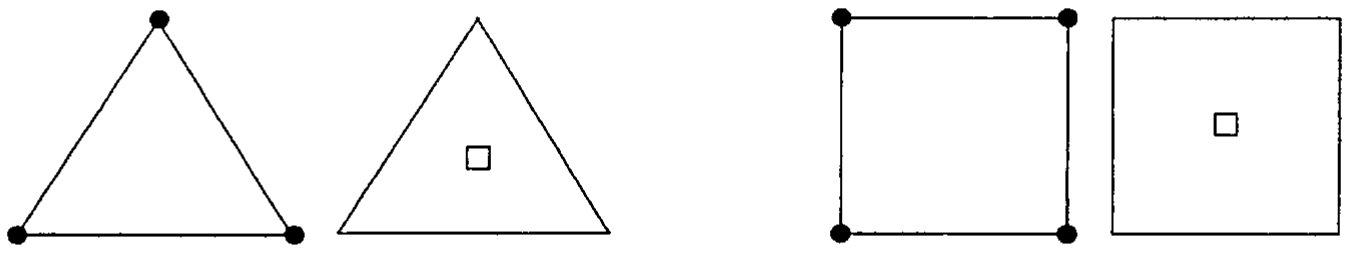
\includegraphics[width=.739\paperwidth]{images/fig-9-3-1.png}
  \caption{分片常值压力与分片线性或双线性速度}\label{fig:9.3.1}
\end{figure}

这类单元一般不满足相容性条件\eqref{eq:9.2.9},还可能发生锁定.例如,设剖分由 \(N\) 个三角形组成,每个三角形都有一条边在 \(\partial\Omega\) 上,且所有三角形共用同一个顶点(见\figref{fig:9.3.2}).此时,\(\boldsymbol{u}_h\) 仅有两个自由度,即唯一的内部顶点上的两个速度分量,而 \(p_h\) 有 \(N-1\) 个自由度,因为压力平均值为零,故比单元数少一个.条件\eqref{eq:9.2.22}于是给出 \(\boldsymbol{u}_h\equiv0\).

\begin{figure}[!htbp]
  \centering
  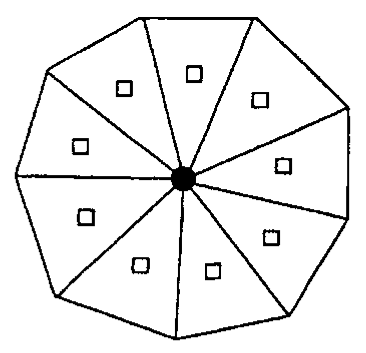
\includegraphics[width=.199\paperwidth]{images/fig-9-3-2.png}
  \caption{导致 \(\boldsymbol{u}_h\) 出现锁定现象的剖分}\label{fig:9.3.2}
\end{figure}

一种部分补救办法是采用所谓的交叉网格剖分.具体做法是将每个三角形 \(K\)(一个\emph{宏单元})分成三个以其重心为公共顶点的子三角形.压力在 \(K\) 上为常数,速度在每个子三角形上为线性函数,并在 \(\overline\Omega\) 上连续(见\figref{fig:9.3.3}).这样的选取消除了锁定现象,但仍不满足相容性条件\eqref{eq:9.2.9},例如见\BookCite{gunzburger1989}{Gunzburger(1989)}第 28 页.

\SourcePage{318}
\begin{figure}[!htbp]
  \centering
  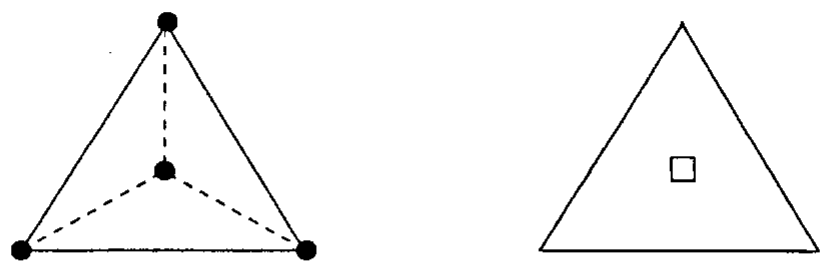
\includegraphics[width=.454\paperwidth]{images/fig-9-3-3.png}
  \caption{(交叉网格 \(\mathbb P_1\))--\(\mathbb P_0\) 单元}\label{fig:9.3.3}
\end{figure}

\figref{fig:9.3.1}右侧的分片 \(\mathbb Q_1\)--\(\mathbb Q_0\) 单元也未通过相容性检验.例如,设 \(\Omega\) 是边与坐标轴平行的矩形,并将它均匀剖分成矩形单元.可证明棋盘格模态在相邻单元上交替取 \(1\) 和 \(-1\)(必要时再减去平均值),由此得到的 \(p_h^*\in Q_h\) 确实是一个伪压力模态(见\BookCite{girault-raviart1986}{Girault 和 Raviart(1986)}第 160 页).

采用\figref{fig:9.3.4}左侧所示的交叉网格剖分,可以滤除该模态.用 \(\mathcal T_h\) 中任一平行四边形 \(K\)(宏单元)的两条对角线,将它分成四个三角形.相应空间是稳定的,并且有以下误差估计(见\BookCite{brezzi-fortin1991}{Brezzi 和 Fortin(1991)}第 VI.5.4 节)：
\begin{equation}\label{eq:9.3.5}
  \|\boldsymbol{u}-\boldsymbol{u}_h\|+\|p-p_h\|_0
       \le Ch(\|\boldsymbol{u}\|_2+\|p\|_1),
\end{equation}
其中 \(\|\cdot\|_s\) 是 \(s\) 阶 Sobolev 范数(见第~\ref{sec:1.2}~节),\(h\) 是宏单元直径的最大值.误差估计\eqref{eq:9.3.5}由\eqref{eq:9.2.11}、\eqref{eq:9.2.12}、定理~\ref{thm:3.4.2}以及估计\eqref{eq:3.5.24}得到,其中默认右端的两个范数均有意义.

\begin{figure}[!htbp]
  \centering
  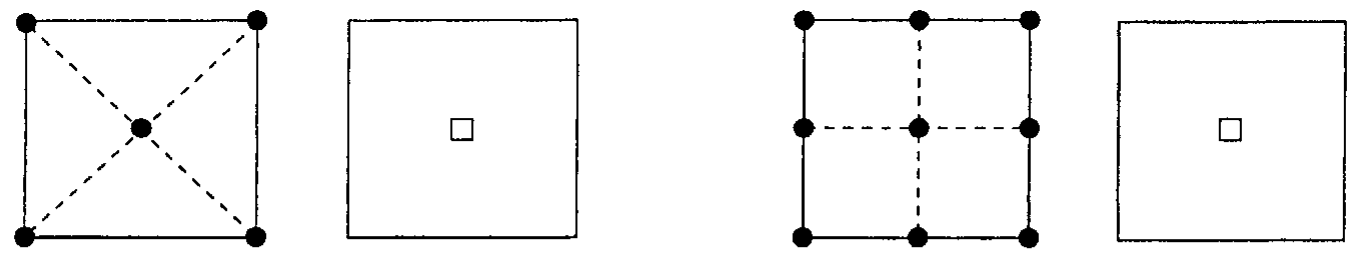
\includegraphics[width=.743\paperwidth]{images/fig-9-3-4.png}
  \caption{(交叉网格 \(\mathbb P_1\))--\(\mathbb Q_0\) 单元(左)和(交叉网格 \(\mathbb Q_1\))--\(\mathbb Q_0\) 单元(右)}\label{fig:9.3.4}
\end{figure}

另一种稳定化办法采用\figref{fig:9.3.4}右侧的宏单元.将每个平行四边形分成四个以其重心为公共顶点的平行四边形,然后在每个子单元上使用 \(\mathbb Q_1\) 多项式.这样的逼近稳定,且具有一阶收敛性(见\BookCite{gunzburger1989}{Gunzburger(1989)}第 30 页).

避免不稳定性的另一种办法是用更丰富的空间逼近速度.这里指出,\(\mathbb P_2\)--\(\mathbb P_0\) 和 \(\mathbb Q_2\)--\(\mathbb Q_0\) 单元都是稳定的,并且都具有一阶收敛性(\BookCite{fortin1972}{Fortin(1972)}).

为获得二阶精度,必须用分片线性多项式逼近压力.不过,\(\mathbb P_2\)--\(\mathbb P_1\) 单元,即在\eqref{eq:9.3.4}中取 \(k=2\) 和 \(m=1\) 所得的单元,仍不稳定(例如,见\BookCite{brezzi-fortin1991}{Brezzi 和 Fortin(1991)}第 231 页).可采用\BookCite{crouzeix-raviart1973}{Crouzeix 和 Raviart(1973)}引入的单元来实现稳定化.这类单元采用间断的分片 \(\mathbb P_1\) \SourcePage{319}压力和分片 \(\mathbb P_2^b(K)\) 速度,其中
\begin{equation}\label{eq:9.3.6}
  \mathbb P_k^b(K):=\{v=p_k+b\mid p_k\in\mathbb P_k,\
            b\text{ 是 }K\text{ 上的三次泡函数}\},\qquad k\ge1.
\end{equation}
三角形 \(K\) 上的三次\emph{泡函数} \(b\) 是在 \(K\) 的边上为零的三次多项式.因此,任一此类函数都可表示为下式的常数倍：
\begin{equation}\label{eq:9.3.7}
  b_K:=\lambda_1\lambda_2\lambda_3,
\end{equation}
其中 \(\{\lambda_i\mid i=1,2,3\}\) 为线性多项式,各自在 \(K\) 的一条边上为零,在对顶点取值 \(1\).泡函数由其在 \(K\) 的重心处的取值确定.Crouzeix--Raviart 单元稳定,且具有二阶收敛性.\figref{fig:9.3.5}左侧给出了它们的自由度.

Crouzeix--Raviart 单元的一种高阶推广采用间断的分片 \(\mathbb P_{k-1}\) 压力和分片 \(\mathbb P_k+B_{k+1}(K)\) 速度,其中在每个三角形 \(K\) 上,
\begin{equation}\label{eq:9.3.8}
  B_{k+1}(K):=\{v\in\mathbb P_{k+1}\mid v=p_{k-2}b_K,\
                    p_{k-2}\in\mathbb P_{k-2}\},\qquad k\ge2,
\end{equation}
而 \(b_K\) 由\eqref{eq:9.3.7}定义.因此,\(B_{k+1}\) 是 \(K\) 上次数不超过 \(k+1\) 的泡函数空间.这些单元满足相容性条件,且以 \(O(h^k)\) 的速率收敛.证明例如见\BookCite{girault-raviart1986}{Girault 和 Raviart(1986)}第 139 页.

\begin{figure}[!htbp]
  \centering
  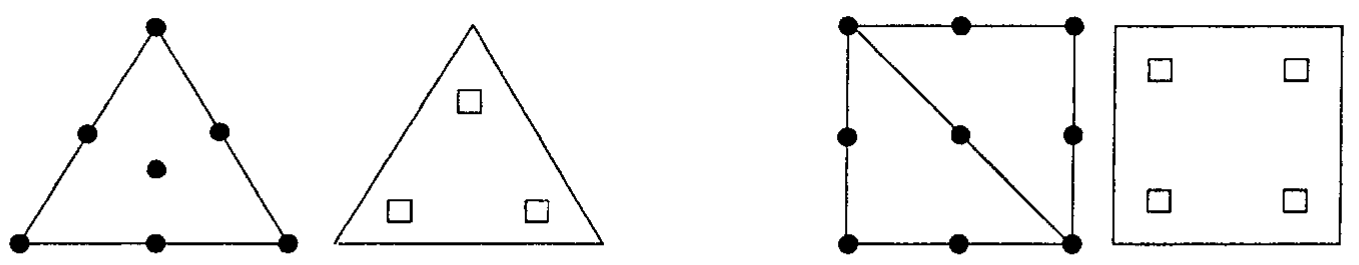
\includegraphics[width=.742\paperwidth]{images/fig-9-3-5.png}
  \caption{Crouzeix--Raviart 单元(左)和 Boland--Nicolaides 单元(右,\(k=2\))}\label{fig:9.3.5}
\end{figure}

另一个很好的例子以平行四边形为基础.采用间断的分片 \(\mathbb Q_{k-1}\) 压力(\(k\ge1\)),再沿各平行四边形的一条对角线将它分成两个三角形,速度在两个三角形上均为 \(\mathbb P_k\) 多项式.\figref{fig:9.3.5}右侧是 \(k=2\) 的例子.这类单元由\BookCite{boland-nicolaides1983}{Boland 和 Nicolaides(1983)}引入,满足相容性条件,且以 \(O(h^k)\) 的速率收敛(另见\BookCite{gunzburger1989}{Gunzburger(1989)}第 36 页).

其他稳定的单元还包括平行六面体剖分上的 \(\mathbb Q_2\)--\(\mathbb P_1\) 单元,其中压力仍是间断的.见\BookCite{girault-raviart1986}{Girault 和 Raviart(1986)}第 156 页.

\subsection{压力连续的有限元}\label{sec:9.3.2}
\SourcePage{320}

为简便起见,本小节也只考察二维情形.若要求有限元压力为连续函数,自然可考虑下列空间：
\begin{equation}\label{eq:9.3.9}
  Q_h=X_h^m\cap L_0^2(\Omega),\quad m\ge1,\qquad
  V_h=(X_h^k\cap H_0^1(\Omega))^2,\quad k\ge1.
\end{equation}

首先指出,所谓的\emph{等阶插值},即速度和压力采用相同多项式次数 \(m=k\),会给出不稳定的逼近.见\BookCite{sani-gresho-lee-griffiths1981}{Sani、Gresho、Lee 和 Griffiths(1981)}、\BookCite{sani-gresho-lee-griffiths-engelman1981}{Sani、Gresho、Lee、Griffiths 和 Engelman(1981)}以及\BookCite{brezzi-fortin1991}{Brezzi 和 Fortin(1991)}第 210 页.

\BookCite{taylor-hood1973}{Taylor 和 Hood(1973)}提出的单元对应\eqref{eq:9.3.9}中 \(m=1\)、\(k=2\) 的选择.这类单元稳定,并以最优速率收敛,即
\begin{equation}\label{eq:9.3.10}
  \|\boldsymbol{u}-\boldsymbol{u}_h\|+\|p-p_h\|_0
     \le Ch^s(\|\boldsymbol{u}\|_{s+1}+\|p\|_s),\qquad s=1,2,
\end{equation}
只要解具有足够的正则性,使右端的范数有意义(例如,见\BookCite{girault-raviart1986}{Girault 和 Raviart(1986)}第 176 页).这一结论对三角形单元和平行六面体型单元均成立.\BookCite{brezzi-falk1991}{Brezzi 和 Falk(1991)}分析了高阶 Taylor--Hood 单元,即\eqref{eq:9.3.9}中取 \(m=k-1\)、\(k\ge3\) 的情形.\figref{fig:9.3.6}给出 \(m=1\)、\(k=2\) 时的自由度.

\begin{figure}[!htbp]
  \centering
  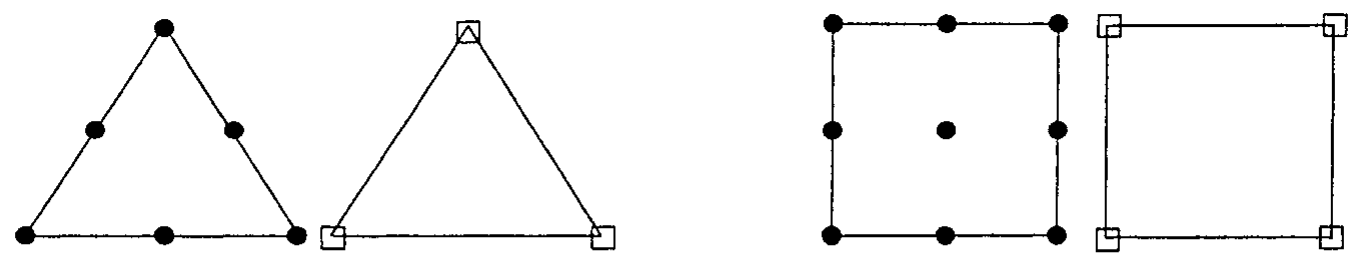
\includegraphics[width=.745\paperwidth]{images/fig-9-3-6.png}
  \caption{低阶 Taylor--Hood 三角形单元(左)和平行四边形单元(右)}\label{fig:9.3.6}
\end{figure}

另一种做法从由三角形 \(K\) 组成的剖分 \(\mathcal T_h\) 出发.压力在每个 \(K\) 上为线性函数,速度在 \(K\) 的三个以重心为公共顶点的子三角形上分片线性(见\figref{fig:9.3.7}左侧).为简便起见,记为(交叉网格 \(\mathbb P_1\))--\(\mathbb P_1\) 单元.这种选取满足相容性条件,相应的有限元解关于 \(h\) 一阶收敛(见\BookCite{pironneau1988}{Pironneau(1988)}第 107 页).

类似的思想产生了所谓的 \((\mathbb P_1\text{ iso }\mathbb P_2)\)--\(\mathbb P_1\) 单元,由\BookCite{bercovier-pironneau1979}{Bercovier 和 Pironneau(1979)}提出,见\figref{fig:9.3.7}右侧.压力空间仍相同,速度在 \(K\) 的四个子三角形上为线性函数,这四个子三角形由连接 \(K\) 各边的中点得到.此离散稳定,且具有一阶收敛性.\SourcePage{321}这种命名是因为其自由度与 \(\mathbb P_2\)--\(\mathbb P_1\) Taylor--Hood 单元的自由度相同(见\figref{fig:9.3.6}左侧).类似地,当 \(\mathcal T_h\) 由平行四边形组成时,可以考察 \((\mathbb Q_1\text{ iso }\mathbb Q_2)\)--\(\mathbb Q_1\) 单元.

\begin{figure}[!htbp]
  \centering
  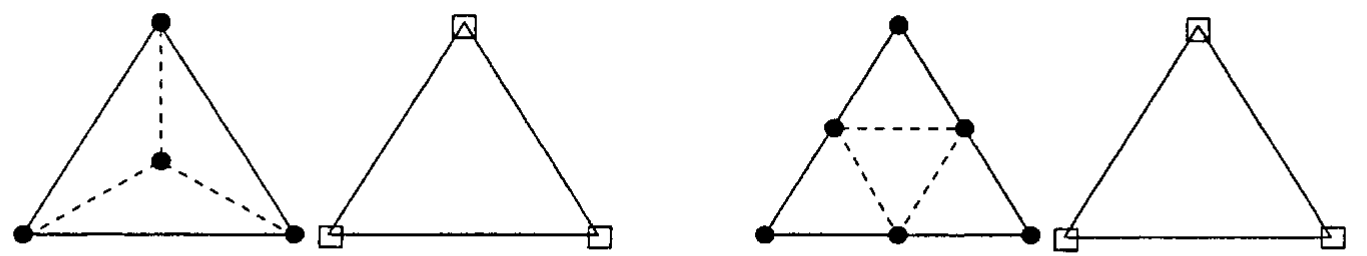
\includegraphics[width=.746\paperwidth]{images/fig-9-3-7.png}
  \caption{(交叉网格 \(\mathbb P_1\))--\(\mathbb P_1\) 单元(左)和 \((\mathbb P_1\text{ iso }\mathbb P_2)\)--\(\mathbb P_1\) 单元(右)}\label{fig:9.3.7}
\end{figure}

最后介绍所谓的 \emph{mini 单元},由\BookCite{arnold-brezzi-fortin1984}{Arnold、Brezzi 和 Fortin(1984)}引入.压力仍为分片 \(\mathbb P_1\) 函数,而速度为分片 \(\mathbb P_1^b\) 函数(见\eqref{eq:9.3.6}).这种选取稳定,并且一阶收敛(见\figref{fig:9.3.8}).mini 单元与\figref{fig:9.3.7}左侧的(交叉网格 \(\mathbb P_1\))--\(\mathbb P_1\) 单元十分相似.事实上,后者将 \(K\) 上在 \(\partial K\) 处为零的三次泡函数 \(b\),换成了同样在 \(\partial K\) 上为零的函数 \(\psi\in C^0(K)\).\(\psi\) 在以 \(K\) 的重心为公共顶点的三个子三角形上分别为线性函数.这两类单元具有相同的稳定性和收敛性质.

\begin{figure}[!htbp]
  \centering
  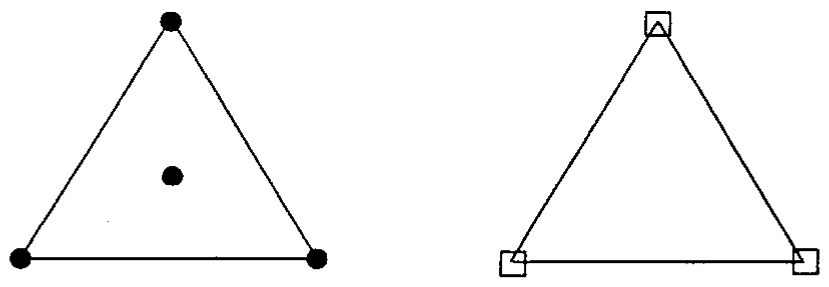
\includegraphics[width=.453\paperwidth]{images/fig-9-3-8.png}
  \caption{mini 单元}\label{fig:9.3.8}
\end{figure}

应用中还使用过许多其他有限元空间,例如速度非协调的单元以及基于降阶积分的单元.有兴趣的读者可参见\BookCite{girault-raviart1986}{Girault 和 Raviart(1986)}及\BookCite{brezzi-fortin1991}{Brezzi 和 Fortin(1991)}.

\section{稳定化方法}\label{sec:9.4}

若采用不满足相容性条件\eqref{eq:9.2.9}的空间对 \(V_h,Q_h\) 来构造鞍点问题\eqref{eq:9.1.11}的逼近\eqref{eq:9.2.4},离散解就可能受到伪压力模态的影响.可按多种准则对它作稳定化处理.

\SourcePage{322}第~\ref{sec:9.3}~节已经看到,有时采用交叉网格剖分,可以使一般剖分上原本不稳定的有限元变得稳定.

另一种稳定化办法并不依赖特殊剖分,而是略微修改\eqref{eq:9.2.4},并相应修改其代数方程组\eqref{eq:9.2.14}.这类方法通常旨在放宽不可压缩性约束,因此会改变\eqref{eq:9.2.4}的第二组方程.抽象地说,稳定化问题为
\begin{equation}\label{eq:9.4.1}
  \left\{
  \begin{aligned}
    &\text{求 }\boldsymbol{u}_h\in V_h,\ p_h\in Q_h,\ \text{使}\\
    &a(\boldsymbol{u}_h,\boldsymbol{v}_h)+b(\boldsymbol{v}_h,p_h)=(\boldsymbol{f},\boldsymbol{v}_h)
          &&\forall\,\boldsymbol{v}_h\in V_h,\\
    &b(\boldsymbol{u}_h,q_h)=\Phi_h(q_h)&&\forall\,q_h\in Q_h,
  \end{aligned}
  \right.
\end{equation}
其中稳定项 \(\Phi_h\) 线性地依赖于试验函数 \(q_h\),也可以依赖 \(\boldsymbol{u}_h\)、\(p_h\)、\(\boldsymbol{f}\) 及 \(h\).为简便起见,以下只考察二维问题.

\BookCite{brezzi-pitkaranta1984}{Brezzi 和 Pitkäranta(1984)}给出了第一个例子,取
\begin{equation}\label{eq:9.4.2}
  \Phi_h(q_h):=\sum_{K\in\mathcal T_h}h_K^2\int_K\nabla p_h\cdot\nabla q_h.
\end{equation}
这里仍以 \(\mathcal T_h\) 表示由三角形 \(K\) 构成的有限元剖分,\(h_K\) 是 \(K\) 的直径.第~\ref{sec:9.3.2}~节已经看到,若 \(\Phi_h\equiv0\),则\eqref{eq:9.3.9}中 \(m=k=1\) 的选择,即对压力和速度都使用连续分片线性多项式,会给出不稳定的逼近.把\eqref{eq:9.4.2}代入\eqref{eq:9.4.1},则得到稳定且一阶收敛的逼近.直观上,由于有 \(\Phi_h(q_h)\) 这一项,至少在\eqref{eq:9.4.2}中以 \(h\) 代替 \(h_K\) 时,可以把\eqref{eq:9.4.1}看作下列修正连续性方程的逼近：
\begin{equation}\label{eq:9.4.3}
  \operatorname{div}\boldsymbol{u}=h^2\Delta p,
\end{equation}
其中压力 \(p\) 满足齐次 Neumann 边界条件.关于这一方法的分析,另见\BookCite{brezzi-douglas1988}{Brezzi 和 Douglas(1988)}.

后来,\BookCite{hughes-franca-balestra1986}{Hughes、Franca 和 Balestra(1986)}建议,对于连续压力空间,采用
\begin{equation}\label{eq:9.4.4}
  \Phi_h(q_h):=\delta\sum_K h_K^2\int_K
      (a_0\boldsymbol{u}_h-\nu\Delta\boldsymbol{u}_h+\nabla p_h-\boldsymbol{f})\cdot\nabla q_h,
\end{equation}
并证明当 \(0<\delta\le C_I\) 时,方法是稳定的,其中 \(C_I\) 是一个适当常数.这一做法类似于第~\ref{sec:8.3.2}~节针对定常对流--扩散方程考察的流线迎风/Petrov--Galerkin(SUPG)法.若按\eqref{eq:9.3.9}取 \(m=k\),则速度和压力都以 \(O(h^k)\) 收敛.这时,在微分方程层次上,若所有 \(K\in\mathcal T_h\) 的 \(h_K\) 都等于 \(h\),连续性方程改为
\SourcePage{323}
\[
  \operatorname{div}\boldsymbol{u}
    =\delta h^2\operatorname{div}(a_0\boldsymbol{u}-\nu\Delta\boldsymbol{u}+\nabla p-\boldsymbol{f}).
\]
由\eqref{eq:9.1}可知,右端恒为零.实践中,参数 \(\delta\) 不能太小,否则无法消除寄生模态.另一方面,\(\delta\) 过大又会使 \(\partial\Omega\) 附近的压力场逼近不佳.还要注意,\eqref{eq:9.4.4}给\eqref{eq:9.2.4}引入了非对称扰动.

另一种选择是用
\begin{equation}\label{eq:9.4.5}
  \Phi_h(q_h):=\delta\sum_K h_K^2\left\{
     \int_K(a_0\boldsymbol{u}_h+\nabla p_h-\boldsymbol{f})\cdot\nabla q_h
     -\int_{\partial K\cap\partial\Omega}\nu\Delta\boldsymbol{u}_h\cdot\boldsymbol{n}\,q_h
    \right\}
\end{equation}
代替\eqref{eq:9.4.4}(见\BookCite{brezzi-douglas1988}{Brezzi 和 Douglas(1988)}).在各单元取相同权重时,对无散度向量 \(\boldsymbol{u}\),若 \(\Delta\boldsymbol{u}\) 连续,则\eqref{eq:9.4.4}和\eqref{eq:9.4.5}一致.这可由 Green 公式\eqref{eq:5.1.5}得到.与\eqref{eq:9.4.4}相比,\eqref{eq:9.4.5}的好处是,矩阵\eqref{eq:9.2.16}的扰动中,涉及 \(\boldsymbol{u}_h\) 的自由度仅限于与边界单元有关的那些自由度.

更一般的办法是同时扰动连续性方程和动量方程.稳定化问题为
\begin{equation}\label{eq:9.4.6}
  \left\{
  \begin{aligned}
    &\text{求 }\boldsymbol{u}_h\in V_h,\ p_h\in Q_h,\ \text{使}\\
    &a(\boldsymbol{u}_h,\boldsymbol{v}_h)+b(\boldsymbol{v}_h,p_h)
       =(\boldsymbol{f},\boldsymbol{v}_h)-\Psi_h^{(\rho)}(\boldsymbol{v}_h)
            &&\forall\,\boldsymbol{v}_h\in V_h,\\
    &b(\boldsymbol{u}_h,q_h)=\Phi_h(q_h)&&\forall\,q_h\in Q_h,
  \end{aligned}
  \right.
\end{equation}
其中 \(\Phi_h(q_h)\) 由\eqref{eq:9.4.4}给出,且
\[
  \begin{aligned}
  \Psi_h^{(\rho)}(\boldsymbol{v}_h):={}&\delta\sum_K h_K^2\int_K
      (a_0\boldsymbol{u}_h-\nu\Delta\boldsymbol{u}_h+\nabla p_h-\boldsymbol{f})\\
      &\hspace{9em}\cdot(\rho a_0\boldsymbol{v}_h-\rho\nu\Delta\boldsymbol{v}_h),
  \end{aligned}
\]
\(\rho\) 是一个参数,通常取 \(-1,0,1\),且 \(\delta>0\).

当 \(\rho=0\) 时,这一方法与 SUPG 法\eqref{eq:9.4.4}一致.当 \(\rho=-1\) 时,称为 Galerkin/最小二乘(GALS)法(\BookCite{hughes-franca1987}{Hughes 和 Franca(1987)}),所得方程组对称.\(\rho=1\) 的情形由\BookCite{douglas-wang1989}{Douglas 和 Wang(1989)}提出,所得方程组不对称.将连续性方程反号后,其双线性形式为半正定,并在更一般的条件下保持稳定.事实上,有下列结果(\BookCite{franca-stenberg1991}{Franca 和 Stenberg(1991)}).

\begin{theorem}[]{9.4.1}
设 \(V_h=(X_h^k\cap H_0^1(\Omega))^2\)、\(Q_h=Y_h^m\cap L_0^2(\Omega)\),其中 \(k\ge2\)、\(m\ge0\).对于 SUPG 和 GALS 法,即分别取 \(\rho=0\) 和 \(\rho=-1\),再假设
\SourcePage{324}
\begin{equation}\label{eq:9.4.7}
  0<\delta<C_I,
\end{equation}
其中 \(C_I\) 是适当常数.则\eqref{eq:9.4.6}给出稳定解,并且有下列最优收敛结果：
\begin{equation}\label{eq:9.4.8}
  \|\boldsymbol{u}-\boldsymbol{u}_h\|+\|p-p_h\|_0
       \le C(h^k\|\boldsymbol{u}\|_{k+1}+h^{m+1}\|p\|_{m+1}).
\end{equation}
当 \(k=1\) 时,只要对某个 \(m\ge1\) 取 \(Q_h=X_h^m\cap L_0^2(\Omega)\),使 \(Q_h\subset C^0(\overline\Omega)\),同样的结论依然成立.
\end{theorem}

\eqref{eq:9.4.7}中的 \(C_I\) 可能很小.事实上,其取值受逆不等式\eqref{eq:6.3.21}中的常数约束.

值得注意的是,有些有限元对问题\eqref{eq:9.2.4}不稳定,用于扰动后问题\eqref{eq:9.4.6}时却是稳定的.其中包括 \(\mathbb P_1\)--\(\mathbb P_1\) 和 \(\mathbb Q_1\)--\(\mathbb Q_1\) 单元(见\figref{fig:9.4.1}).

\begin{figure}[!htbp]
  \centering
  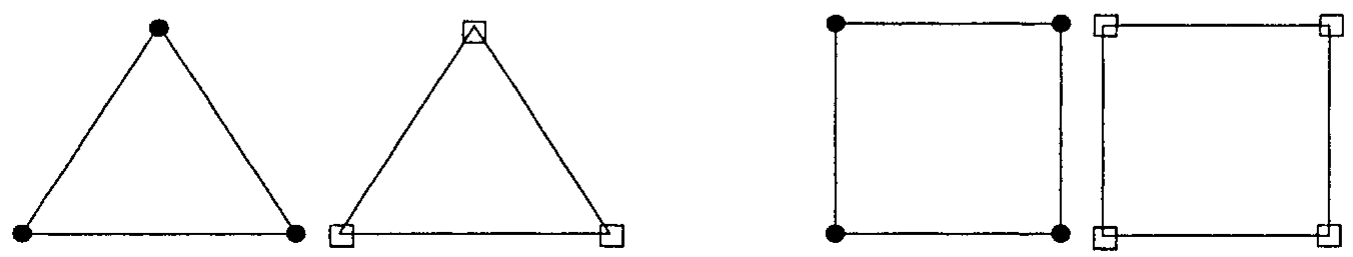
\includegraphics[width=.739\paperwidth]{images/fig-9-4-1.png}
  \caption{满足定理~\ref{thm:9.4.1}假设的有限元示例}\label{fig:9.4.1}
\end{figure}

\begin{note}\NumberedNote{note:9.4.1}
对于分片线性速度,或在矩形网格上的分片双线性速度,对所有 \(K\in\mathcal T_h\) 都有 \(\Delta\boldsymbol{v}_h|_K=0\).因此,在这一情形下,若再假定 \(a_0=0\),则本节迄今考察的各方法(\eqref{eq:9.4.2}除外)彼此一致.\hfill\(\square\)
\end{note}

前一个定理不适用于最低阶单元
\begin{equation}\label{eq:9.4.9}
  V_h=(X_h^1\cap H_0^1(\Omega))^2,\qquad Q_h=Y_h^0\cap L_0^2(\Omega)
\end{equation}
(见\figref{fig:9.3.1}).这类单元在一般剖分上仍可能有伪模态(见第~\ref{sec:9.3.1}~节).在这种情形下,一种稳定化方法如下：
\begin{equation}\label{eq:9.4.10}
  \left\{
  \begin{aligned}
    &\text{求 }\boldsymbol{u}_h\in V_h,\ p_h\in Q_h,\ \text{使}\\
    &a(\boldsymbol{u}_h,\boldsymbol{v}_h)+b(\boldsymbol{v}_h,p_h)=(\boldsymbol{f},\boldsymbol{v}_h)
       &&\forall\,\boldsymbol{v}_h\in V_h,\\
    &b(\boldsymbol{u}_h,q_h)=\delta\sum_{\sigma\in\Gamma_h}h_\sigma
          \int_\sigma[p_h]_\sigma[q_h]_\sigma &&\forall\,q_h\in Q_h,
  \end{aligned}
  \right.
\end{equation}
其中 \(\delta>0\) 是适当常数,\(\Gamma_h\) 是剖分中除边界 \(\partial\Omega\) 上的边以外的所有边的集合,\(h_\sigma\) 是 \(\sigma\) 的\SourcePage{325}长度.最后,对任意 \(q_h\in Q_h\),\([q_h]_\sigma\) 表示它跨边 \(\sigma\) 的跳跃.对于所有 \(\delta>0\),这一方法都给出稳定且一阶收敛的解,即
\[
  \|\boldsymbol{u}-\boldsymbol{u}_h\|+\|p-p_h\|_0\le Ch(\|\boldsymbol{u}\|_2+\|p\|_1)
\]
(\BookCite{kechkar-silvester1992}{Kechkar 和 Silvester(1992)}).

\eqref{eq:9.4.10}的代数表述给出如下对称、非奇异的方程组：
\begin{equation}\label{eq:9.4.11}
  \begin{pmatrix}A&B^T\\B&-\delta D\end{pmatrix}
     \begin{pmatrix}\boldsymbol{u}\\\boldsymbol{p}\end{pmatrix}
       =\begin{pmatrix}\boldsymbol{f}\\0\end{pmatrix},
\end{equation}
其中 \(D\) 为对称半正定矩阵,元素为
\begin{equation}\label{eq:9.4.12}
  D_{ij}:=\sum_{\sigma\in\Gamma_h}h_\sigma\int_\sigma[\psi_i]_\sigma[\psi_j]_\sigma.
\end{equation}
从代数上看,记\eqref{eq:9.4.11}中的矩阵为 \(S_\delta\),则可分解为
\[
  S_\delta=
  \begin{pmatrix}A&0\\B&I\end{pmatrix}
  \begin{pmatrix}A^{-1}&0\\0&-BA^{-1}B^T-\delta D\end{pmatrix}
  \begin{pmatrix}A&B^T\\0&I\end{pmatrix}.
\]
因此,由 Sylvester 惯性定律,\(S_\delta\) 的正、负特征值个数与第二个因子的相同,即有 \(N_h\) 个正特征值和 \(K_h\) 个负特征值.回顾一下,若 \(\ker B^T\ne\{0\}\),则\eqref{eq:9.2.16}中的矩阵 \(S\) 有 \(N_h\) 个正特征值,其余 \(K_h\) 个特征值为负或为零.

若剖分由\emph{宏单元}组成,且每个宏单元含四个三角形或四边形(见\figref{fig:9.4.2}),便可简化\eqref{eq:9.4.10}.其中关于 \(\sigma\in\Gamma_h\) 的求和可只取每个宏单元的内部边.简化后的格式与\eqref{eq:9.4.10}具有相同的稳定性和收敛性,而 \(D\) 的带宽更小.

\begin{figure}[!htbp]
  \centering
  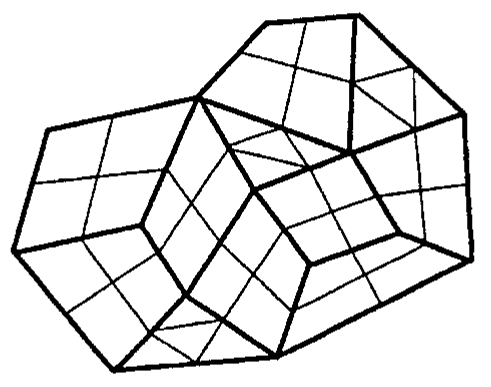
\includegraphics[width=.268\paperwidth]{images/fig-9-4-2.png}
  \caption{\(\Omega\) 的宏单元剖分}\label{fig:9.4.2}
\end{figure}

\begin{note}\NumberedNote{note:9.4.2}{\heiti(稳定化与泡函数)}
\BookCite{baiocchi-brezzi-franca1993}{Baiocchi、Brezzi 和 Franca(1993)}指出,在有限元空间中加入泡函数,可以得到一种在形式上类似于前述方法的稳定化方法(另见\SourcePage{326}\BookCite{pierre1988}{Pierre(1988}、\BookCite{pierre1989}{1989)}及\BookCite{bank-welfert1990}{Bank 和 Welfert(1990)}).类似的结论也适用于第~\ref{sec:8.3.2}~节引入的对流--扩散问题稳定化方法(见第~\ref{sec:8.3.3}~节).

用抽象的方式,可将采用泡函数空间的有限维方法表述如下.令
\[
  \mathcal V_h^b:=\mathcal U_h\oplus\mathcal B,
\]
其中 \(\mathcal U_h\) 是标准有限元空间,\(\mathcal B\) 是泡函数空间.例如,对\figref{fig:9.3.8}中的 mini 单元,有
\begin{equation}\label{eq:9.4.13}
  \mathcal U_h=(X_h^1\cap H_0^1(\Omega))^2\times(X_h^1\cap L_0^2(\Omega)),
      \qquad \mathcal B|_K=(B_3(K))^2\times\{0\}
\end{equation}
(见\eqref{eq:9.3.8}).然后,以 \(\mathcal A(\cdot,\cdot)\) 表示边值问题对应的双线性形式.有限维问题可表述为
\begin{equation}\label{eq:9.4.14}
  \begin{aligned}
    \text{求 }\boldsymbol{u}_h+\boldsymbol{u}_B\in\mathcal V_h^b,\quad\text{使}\quad
     \mathcal A(\boldsymbol{u}_h+\boldsymbol{u}_B,\boldsymbol{v}_h+\boldsymbol{v}_B)
       &=\mathcal F(\boldsymbol{v}_h+\boldsymbol{v}_B)\\
       &\qquad\forall\,\boldsymbol{v}_h\in\mathcal U_h,\ \boldsymbol{v}_B\in\mathcal B.
  \end{aligned}
\end{equation}
特别地,取 \(\boldsymbol{v}_h=0\),有
\[
  \mathcal A(\boldsymbol{u}_h+\boldsymbol{u}_B,\boldsymbol{v}_B)
       =\mathcal F(\boldsymbol{v}_B)\qquad\forall\,\boldsymbol{v}_B\in\mathcal B.
\]
逐单元计算 \(\boldsymbol{u}_B\),得到
\begin{equation}\label{eq:9.4.15}
  \boldsymbol{u}_B=\boldsymbol{\Phi}(\boldsymbol{f},\boldsymbol{u}_h),
\end{equation}
其中 \(\boldsymbol{\Phi}\) 是适当的映射.现在,在\eqref{eq:9.4.14}中取 \(\boldsymbol{v}_B=0\),可得
\begin{equation}\label{eq:9.4.16}
  \mathcal A(\boldsymbol{u}_h,\boldsymbol{v}_h)
    =\mathcal F(\boldsymbol{v}_h)-\mathcal A(\boldsymbol{\Phi}(\boldsymbol{f},\boldsymbol{u}_h),\boldsymbol{v}_h)
         \qquad\forall\,\boldsymbol{v}_h\in\mathcal U_h .
\end{equation}
这一问题就是在原空间 \(\mathcal U_h\) 上表述的 Galerkin 逼近.右端第二项可以看作旨在使解 \(\boldsymbol{u}_h\) 稳定的扰动.以 mini 单元为例,泡函数产生的效果可视为在空间 \(\mathcal U_h\) 上作 GALS 逼近.\hfill\(\square\)
\end{note}

\begin{note}\NumberedNote{note:9.4.3}
稳定化问题\eqref{eq:9.4.6}可写成类似于第~\ref{sec:8.3.2}~节对流--扩散方程的方法.事实上,若将 Stokes 算子和右端写为
\begin{equation}\label{eq:9.4.17}
  L(\boldsymbol{w},r):=\begin{pmatrix}a_0\boldsymbol{w}-\nu\Delta\boldsymbol{w}+\nabla r\\
                \operatorname{div}\boldsymbol{w}\end{pmatrix},
   \qquad \boldsymbol{f}^*:=\begin{pmatrix}\boldsymbol{f}\\0\end{pmatrix},
\end{equation}
则 \(L\) 关于 \(L^2(\Omega)\) 内积的对称部分和斜对称部分为
\SourcePage{327}
\begin{equation}\label{eq:9.4.18}
  L_S(\boldsymbol{w},r):=\begin{pmatrix}a_0\boldsymbol{w}-\nu\Delta\boldsymbol{w}\\0\end{pmatrix},
   \qquad L_{SS}(\boldsymbol{w},r):=\begin{pmatrix}\nabla r\\\operatorname{div}\boldsymbol{w}\end{pmatrix}.
\end{equation}
于是,可引入如下稳定化问题：求 \((\boldsymbol{u}_h,p_h)\in V_h\times Q_h\),使
\begin{equation}\label{eq:9.4.19}
  \begin{aligned}
    &a(\boldsymbol{u}_h,\boldsymbol{v}_h)+b(\boldsymbol{v}_h,p_h)-b(\boldsymbol{u}_h,q_h)\\
    &\quad+\delta\sum_{K\in\mathcal T_h}
        (L(\boldsymbol{u}_h,p_h)-\boldsymbol{f}^*,h_K^2(L_{SS}+\rho L_S)(\boldsymbol{v}_h,q_h))_K\\
    &\quad=(\boldsymbol{f},\boldsymbol{v}_h)
  \end{aligned}
\end{equation}
对每个 \((\boldsymbol{v}_h,q_h)\in V_h\times Q_h\) 成立.这与\eqref{eq:9.4.6}基本相同,事实上只在\eqref{eq:9.4.19}左端增加了稳定项
\[
  \delta\sum_{K\in\mathcal T_h}h_K^2(\operatorname{div}\boldsymbol{u}_h,\operatorname{div}\boldsymbol{v}_h)_K.
\]

注意,对流--扩散方程的 GALS 法对应 \(\rho=1\),Stokes 问题的 GALS 法则对应 \(\rho=-1\).这一名称对应的参数发生变化,是因为 GALS 法最初从 Stokes 算子的对称形式出发,即
\[
  L^*(\boldsymbol{w},r):=\begin{pmatrix}a_0\boldsymbol{w}-\nu\Delta\boldsymbol{w}+\nabla r\\
                    -\operatorname{div}\boldsymbol{w}\end{pmatrix}
\]
(见\BookCite{hughes-franca1987}{Hughes 和 Franca(1987)}),再从方程左端减去“最小二乘”项
\[
  \delta\sum_K h_K^2(a_0\boldsymbol{u}_h-\nu\Delta\boldsymbol{u}_h+\nabla p_h-\boldsymbol{f},\
                    a_0\boldsymbol{v}_h-\nu\Delta\boldsymbol{v}_h+\nabla q_h)_K .
\]
这对应于\eqref{eq:9.4.19}中 \(\rho=-1\) 的选择.事实上,对 Stokes 问题而言,将“最小二乘法”这一名称用于\eqref{eq:9.4.6}中 \(\rho=1\) 的 Douglas--Wang 法会更贴切.\hfill\(\square\)
\end{note}

\section{谱方法逼近}\label{sec:9.5}

这类逼近的特点是,试验函数和近似解都用高次代数多项式表示.为简便起见,假定 \(\Omega=(-1,1)^d\),\(d=2,3\).对于更一般的区域,需要采用区域分解方法,例如见第~\ref{sec:6.4}~节.

先逼近问题\eqref{eq:9.1.6},取
\begin{equation}\label{eq:9.5.1}
  V_N:=(\mathbb Q_N^0)^d,\qquad
  V_{\mathrm{div},N}:=\{\boldsymbol{v}_N\in V_N\mid\operatorname{div}\boldsymbol{v}_N=0\},
\end{equation}
\SourcePage{328}其中,仍以 \(\mathbb Q_N^0\) 记关于每个变量 \(x_i\)(\(i=1,\ldots,d\))的次数均不超过 \(N\)、在 \(\partial\Omega\) 上为零的代数多项式空间.此时,Galerkin 逼近\eqref{eq:9.2.1}写成
\begin{equation}\label{eq:9.5.2}
  \text{求 }\boldsymbol{u}_N\in V_{\mathrm{div},N},\quad\text{使}\quad
      a(\boldsymbol{u}_N,\boldsymbol{v}_N)=(\boldsymbol{f},\boldsymbol{v}_N)
       \qquad\forall\,\boldsymbol{v}_N\in V_{\mathrm{div},N}.
\end{equation}
这一问题存在唯一解,解是稳定的,并满足\eqref{eq:9.2.3}的收敛结论,只需相应改变记号.为得到关于 \(N^{-1}\) 的收敛阶,需要估计\eqref{eq:9.2.3}右端的下确界.为此,使用\BookCite{sacchilandriani-vandeven1989}{Sacchi Landriani 和 Vandeven(1989)}证明的下列结果.

\begin{theorem}[]{9.5.1}
对任意 \(s\ge1\),都存在与 \(N\) 无关的常数 \(C\),使对所有 \(\boldsymbol{v}\in(H^s(\Omega))^d\cap V_{\mathrm{div}}\),有
\begin{equation}\label{eq:9.5.3}
  \inf_{\boldsymbol{v}_N\in V_{\mathrm{div},N}}\|\boldsymbol{v}-\boldsymbol{v}_N\|
    \le CN^{1-s}\|\boldsymbol{v}\|_s.
\end{equation}
\end{theorem}

\begin{proof}
只考察二维情形(\(d=2\)).首先,对任意 \(\boldsymbol{v}\in V_{\mathrm{div}}\),存在{\heiti 流函数} \(\psi\in H^2(\Omega)\),使
\begin{equation}\label{eq:9.5.4}
  \boldsymbol{v}=\operatorname{rot}\psi:=
     \left(\frac{\partial\psi}{\partial x_2},-\frac{\partial\psi}{\partial x_1}\right)
       \qquad\text{在 }\Omega\text{ 内}.
\end{equation}
此外,若 \(\boldsymbol{v}\in(H^s(\Omega))^2\),其中 \(s\ge1\),则 \(\psi\in H^{s+1}(\Omega)\),选定其加性常数后有
\begin{equation}\label{eq:9.5.5}
  \|\psi\|_{s+1}\le C\|\boldsymbol{v}\|_s.
\end{equation}
由于 \(\boldsymbol{v}=0\) 在 \(\partial\Omega\) 上成立,\(\nabla\psi\) 在 \(\partial\Omega\) 上为零.此外,\(\psi\) 只确定到一个加性常数,可以令它在一个边界点处为零,从而它在整个 \(\partial\Omega\) 上恒为零.因此,\(\psi\in H_0^2(\Omega)\),其中
\begin{equation}\label{eq:9.5.6}
  H_0^2(\Omega)=\left\{\varphi\in H^2(\Omega)\ \middle|\
      \varphi=\frac{\partial\varphi}{\partial n}=0\text{ 在 }\partial\Omega\text{ 上}\right\}.
\end{equation}
在这一空间上,可以定义算子 \(P_{2,N}^0\),将任意 \(H_0^2(\Omega)\) 中的函数,按 \(H^2(\Omega)\) 的内积,正交投影到次数不超过 \(N\)、且函数及其法向导数均在 \(\partial\Omega\) 上为零的多项式空间.沿用类似于推导 \(P_{1,N}^0\) 误差估计的论证(见第~\ref{sec:4.5.2}~节),可证明
\begin{equation}\label{eq:9.5.7}
  \|\psi-P_{2,N}^0\psi\|_2
       \le CN^{1-s}\|\psi\|_{s+1}\le CN^{1-s}\|\boldsymbol{v}\|_s,\qquad s\ge1,
\end{equation}
其中最后一个不等式由\eqref{eq:9.5.5}得到.取 \(\boldsymbol{v}_N=\operatorname{rot}(P_{2,N}^0\psi)\),并注意 \(\boldsymbol{v}_N\in V_{\mathrm{div},N}\),即得\eqref{eq:9.5.3}.\hfill\(\square\)
\end{proof}

\SourcePage{329}由\eqref{eq:9.2.3}和\eqref{eq:9.5.3}可知
\begin{equation}\label{eq:9.5.8}
  \|\boldsymbol{u}-\boldsymbol{u}_N\|\le CN^{1-s}\|\boldsymbol{u}\|_s,
\end{equation}
其中假定对某个 \(s\ge1\),有 \(\boldsymbol{u}\in(H^s(\Omega))^d\cap V_{\mathrm{div}}\).得到 \(\boldsymbol{u}_N\) 之后,问题是如何恢复具有同样最优精度的压力场 \(p_N\).这并不容易,不过有些情况下可以做到.特别可参见\BookCite{moser-moin-leonard1983}{Moser、Moin 和 Leonard(1983)}的方法及其推广(见\BookCite{pasquarelli-quarteroni-sacchilandriani1987}{Pasquarelli、Quarteroni 和 Sacchi Landriani(1987)}及\BookCite{pasquarelli1991}{Pasquarelli(1991)}).不过要注意,这一做法采用由 Chebyshev 多项式的线性组合构成的 \(V_{\mathrm{div},N}\) 基(见第~\ref{sec:4.5.1}~节).相应地,\eqref{eq:9.5.2}中的每个积分都要换成采用 Chebyshev 权函数的加权积分(见第~\ref{sec:4.5.1}~节).

一般来说,构造 \(V_{\mathrm{div},N}\) 的基和恢复压力场都比较困难,因此可以直接逼近鞍点问题\eqref{eq:9.1.11}.对这一问题,可以采用谱 Galerkin 法,也可以采用广义 Galerkin 法,后者往往与谱配置法等价.

\subsection{谱 Galerkin 逼近}\label{sec:9.5.1}

令 \(Q_N\) 和 \(V_N\) 分别为 \(L_0^2(\Omega)\) 和 \((H_0^1(\Omega))^d\) 的多项式子空间,考察\eqref{eq:9.1.11}的下列谱逼近：
\begin{equation}\label{eq:9.5.9}
  \left\{
  \begin{aligned}
    &\text{求 }\boldsymbol{u}_N\in V_N,\ p_N\in Q_N,\ \text{使}\\
    &a(\boldsymbol{u}_N,\boldsymbol{v}_N)+b(\boldsymbol{v}_N,p_N)=(\boldsymbol{f},\boldsymbol{v}_N)
         &&\forall\,\boldsymbol{v}_N\in V_N,\\
    &b(\boldsymbol{u}_N,q_N)=0&&\forall\,q_N\in Q_N.
  \end{aligned}
  \right.
\end{equation}
通常,\(V_N\) 取为\eqref{eq:9.5.1}定义的空间,这可以保证速度场具有形如\eqref{eq:9.5.8}的误差估计.相应地,本想取 \(Q_N=M_N\),其中 \(M_N:=\mathbb Q_N\cap L_0^2(\Omega)\).但这种选择不合适,因为 \(V_N,M_N\) 不满足相容性条件\eqref{eq:9.2.9}.因此,需要选取 \(M_N\) 的一个真子空间作为 \(Q_N\).

先定义
\begin{equation}\label{eq:9.5.10}
  S_N:=\{p_N^*\in\mathbb Q_N\mid b(\boldsymbol{v}_N,p_N^*)=0\quad
                  \forall\,\boldsymbol{v}_N\in V_N\},
\end{equation}
即 \(\mathbb Q_N\) 中由所有伪压力模态组成的子空间(见\eqref{eq:9.2.21}).再定义
\begin{equation}\label{eq:9.5.11}
  D_N:=\{\varphi_N\in\mathbb Q_N\mid
          \exists\,\boldsymbol{v}_N\in V_N,\ \operatorname{div}\boldsymbol{v}_N=\varphi_N\},
\end{equation}
即 \(V_N\) 在散度算子下的像.显然,关于 \(L^2(\Omega)\) 内积,\(D_N\) 是 \(S_N\) 在 \(\mathbb Q_N\) 中的正交补.\SourcePage{330}可以完整刻画空间 \(S_N\).先注意,可以取 \(S_N\) 在 \(\mathbb Q_N\) 中的任一补空间作为压力空间 \(Q_N\),即取任一满足
\begin{equation}\label{eq:9.5.12}
  \dim S_N+\dim Q_N=\dim\mathbb Q_N,\qquad S_N\cap Q_N=\{0\}
\end{equation}
的子空间 \(Q_N\subset\mathbb Q_N\),并以选取零平均值代表元的方式固定压力的加性常数.

下列结果刻画了二维逼近的伪模态空间,证明例如见\BookCite{bernardi-maday1992}{Bernardi 和 Maday(1992)}第 126–127 页.

\begin{theorem}[]{9.5.2}
设 \(\Omega=(-1,1)^2\) 且 \(N\ge3\).空间 \(S_N\) 的维数为 \(8\),它的一组基由下列多项式给出：
\begin{equation}\label{eq:9.5.13}
  \begin{gathered}
    1,\quad L_N(x_1),\quad L_N(x_2),\quad L_N(x_1)L_N(x_2),\quad
          L_N'(x_1)L_N'(x_2),\\
    L_N'(x_1)L_{N+1}'(x_2),\quad L_{N+1}'(x_1)L_N'(x_2),\quad
       L_{N+1}'(x_1)L_{N+1}'(x_2),
  \end{gathered}
\end{equation}
其中 \(\{L_k\mid k=0,1,\ldots\}\) 为第~\ref{sec:4.4.1}~节引入的 Legendre 多项式.
\end{theorem}

\begin{proof}
容易证明,\eqref{eq:9.5.13}中的每个函数都属于 \(S_N\).反过来,来证明 \(S_N\) 中任意函数 \(p_N^*\) 都可由上述多项式线性组合得到.注意,\(p_N^*\) 必须满足
\begin{equation}\label{eq:9.5.14}
  \int_\Omega p_N^*\left(\frac{\partial v_{N,1}}{\partial x_1}
                       +\frac{\partial v_{N,2}}{\partial x_2}\right)\mathrm d\boldsymbol{x}=0
        \qquad\forall\,\boldsymbol{v}_N=(v_{N,1},v_{N,2})\in V_N .
\end{equation}
先取 \(\boldsymbol{v}_N=(\varphi_{mn},0)\),再取 \(\boldsymbol{v}_N=(0,\varphi_{mn})\),其中
\[
  \varphi_{mn}(x_1,x_2)=(1-x_1^2)(1-x_2^2)L_m'(x_1)L_n'(x_2),
       \qquad1\le m,n\le N-1.
\]
由\eqref{eq:9.5.14}可得
\begin{equation}\label{eq:9.5.15}
  \begin{aligned}
    \int_\Omega p_N^*(\boldsymbol{x})L_m(x_1)(1-x_2^2)L_n'(x_2)\,\mathrm d\boldsymbol{x}
      &=\int_\Omega p_N^*(\boldsymbol{x})(1-x_1^2)L_m'(x_1)L_n(x_2)\,\mathrm d\boldsymbol{x}\\
      &=0 .
  \end{aligned}
\end{equation}
这里使用了 Legendre 多项式的 Sturm--Liouville 公式(见\eqref{eq:4.4.2})：
\begin{equation}\label{eq:9.5.16}
  \bigl((1-\xi^2)L_k'(\xi)\bigr)'=-k(k+1)L_k(\xi),\qquad -1<\xi<1.
\end{equation}
回顾(见\eqref{eq:6.2.20}),
\begin{equation}\label{eq:9.5.17}
  \varphi_k(\xi):=(1-\xi^2)L_k'(\xi),\qquad1\le k\le N-1,
\end{equation}
是在 \(\xi=\pm1\) 处为零、次数不超过 \(N\) 的一维多项式空间 \(\mathbb P_N^0\) 的一组基.由\eqref{eq:9.5.16}和\eqref{eq:4.4.6}可知,\(\mathbb P_N^0\) 在 \(\mathbb P_N\) 中的正交补由 \(L_N'(\xi)\) 和 \(L_{N+1}'(\xi)\) 张成.因此,由\eqref{eq:9.5.15}可知,\(p_N^*\) 可写成
\SourcePage{331}
\[
  \begin{aligned}
    p_N^*(x_1,x_2)={}&a_0(x_2)+a_N(x_2)L_N(x_1)\\
           &+b_N(x_1)L_N'(x_2)+b_{N+1}(x_1)L_{N+1}'(x_2),
  \end{aligned}
\]
也可写成
\[
  \begin{aligned}
    p_N^*(x_1,x_2)={}&c_0(x_1)+c_N(x_1)L_N(x_2)\\
           &+d_N(x_2)L_N'(x_1)+d_{N+1}(x_2)L_{N+1}'(x_1),
  \end{aligned}
\]
其中 \(a_0,a_N,\ldots,d_N,d_{N+1}\) 是次数不超过 \(N\) 的代数多项式.因此,\(p_N^*\) 可表示为\eqref{eq:9.5.13}中各多项式的线性组合.

还需证明\eqref{eq:9.5.13}中的八个多项式线性无关.为此,只需验证 \(\{1,L_N,L_N',L_{N+1}'\}\) 线性无关.假设
\[
  \alpha_0+\alpha_NL_N+\beta_NL_N'+\beta_{N+1}L_{N+1}'=0.
\]
由积分关系
\[
  \int_{-1}^{\xi}L_k(\eta)\,\mathrm d\eta
    =\frac{L_{k+1}(\xi)-L_{k-1}(\xi)}{2k+1},\qquad -1\le\xi\le1,\quad k\ge1,
\]
可用 \((2N+1)L_N+L_{N-1}'\) 替换 \(L_{N+1}'\).注意,\(L_N\) 与 \(L_N'\) 的奇偶性不同.比较替换后各多项式的次数 \(0,N,N-1,N-2\),容易得到
\(\alpha_0=\alpha_N=\beta_N=\beta_{N+1}=0\).\hfill\(\square\)
\end{proof}

等价地,上述定理表明,\(D_N\) 在 \(\mathbb Q_N\) 中的余维为 \(8\).

非常数伪模态的存在表明,取 \(Q_N=\mathbb Q_N\) 为压力空间不能满足相容性条件.取 \(Q_N=D_N\) 时,该条件当然成立.不过,\eqref{eq:9.2.9}中的最优常数 \(\beta\) 关于 \(N\) 没有一致的正下界.证明这一性质的重要一步依赖于下列结果,其证明见\BookCite{bernardi-maday1992}{Bernardi 和 Maday(1992)}第 130 页.

\begin{lemma}[]{9.5.1}
对任意 \(q_N\in D_N\),存在多项式 \(\boldsymbol{v}_N\in V_N\),使
\begin{align}
  \operatorname{div}\boldsymbol{v}_N&=q_N,\label{eq:9.5.18}\\
  \|\boldsymbol{v}_N\|&\le CN\|q_N\|_0.\label{eq:9.5.19}
\end{align}
\end{lemma}

由这一引理,对每个 \(q_N\in D_N\),可以找到 \(\boldsymbol{v}_N\in V_N\),使
\[
  |b(\boldsymbol{v}_N,q_N)|=
      \left|\int_\Omega q_N\operatorname{div}\boldsymbol{v}_N\,\mathrm d\boldsymbol{x}\right|
        =\int_\Omega q_N^2\,\mathrm d\boldsymbol{x}
        \ge CN^{-1}\|\boldsymbol{v}_N\|\|q_N\|_0.
\]
\SourcePage{332}因此,\((V_N,D_N)\) 满足相容性条件,且 \(\beta\) 的最优值不小于 \(CN^{-1}\).这个结果不能改进,因为在 \(N\to\infty\) 时,找不到一个满足\eqref{eq:9.2.9}且比 \(N^{-1}\) 趋零更慢的 \(\beta\).因此,当 \(V_N=(\mathbb Q_N^0)^2\) 且 \(Q_N=D_N\) 时,Stokes 问题的谱 Galerkin 逼近有
\begin{equation}\label{eq:9.5.20}
  \beta\asymp N^{-1}.
\end{equation}

不过,从能否一致逼近压力的角度看,选择 \(Q_N=D_N\) 作为压力空间并不合适.事实上,\(D_N\) 与多项式 \(L_N'(x_1)L_N'(x_2)\) 等正交,这意味着某些低次多项式无法包含在 \(D_N\) 中.因此,\(D_N\) 不适合用来逼近物理压力空间 \(L_0^2(\Omega)\) 中的所有函数.

\BookCite{bernardi-maday-metivet1987}{Bernardi、Maday 和 Métivet(1987)}给出了一个更合适的选择：取 \(Q_N\) 为 \(\mathbb Q_N\) 中与下列多项式正交的所有多项式所成的空间：
\[
  \begin{gathered}
    1,\quad L_N(x_1),\quad L_N(x_2),\quad L_N(x_1)L_N(x_2),\quad
         A_{N-1}(x_1)A_{N-1}(x_2),\\
    A_{N-1}(x_1)A_N(x_2),\quad A_N(x_1)A_{N-1}(x_2),\quad A_N(x_1)A_N(x_2),
  \end{gathered}
\]
其中
\[
  A_{N-1}:=L_N'-P_{\lfloor\lambda N\rfloor}L_N',\qquad
  A_N:=P_{N-1}L_{N+1}'-P_{\lfloor\lambda N\rfloor}L_{N+1}'.
\]
对任意 \(0<\lambda<1\),\(\lfloor\lambda N\rfloor\) 表示 \(\lambda N\) 的整数部分,\(P_{\lfloor\lambda N\rfloor}\) 表示关于\eqref{eq:4.4.5}所定义的内积到次数不超过 \(\lfloor\lambda N\rfloor\) 的一维多项式空间上的正交投影.

这个选择看上去比较复杂,但从理论上很合适,因为相容性条件成立,且常数 \(\beta\) 与\eqref{eq:9.5.20}具有相同的渐近行为.此外,按上述准则选取的 \(Q_N\) 足够丰富,包含所有次数不超过 \(\lfloor\lambda N\rfloor\) 且平均值为零的多项式.因此,\(Q_N\) 具有最优的逼近性质.事实上,利用\eqref{eq:9.2.12}并结合\eqref{eq:9.5.20},得到下列压力误差估计：
\begin{equation}\label{eq:9.5.21}
  \|p-p_N\|_0\le CN^{2-s}(\|\boldsymbol{u}\|_s+\|p\|_{s-1}),\qquad s\ge2,
\end{equation}
其中假定精确解 \((\boldsymbol{u},p)\) 具有右端所要求的光滑性.注意,\eqref{eq:9.5.21}与最优估计相差一个因子 \(N\),它正是常数 \(\beta\) 的倒数的量级.

\subsection{谱配置逼近}\label{sec:9.5.2}
\SourcePage{333}

用谱方法逼近 Stokes 方程时,通常较多采用配置法.理由之一是\eqref{eq:9.5.9}的右端难以计算,配置法用 Gauss 数值积分代替所有积分,克服了这一困难.

令 \(\Omega=(-1,1)^2\),取整数 \(N\ge3\).以 \(\Omega_N\) 记全部 \((N+1)^2\) 个 Legendre--Gauss--Lobatto 节点(见\eqref{eq:4.5.38}),以 \(\Xi_N\) 记 \(\Omega_N\) 中属于 \(\Omega\) 内部的 \((N-1)^2\) 个节点,以 \(\Sigma_N\) 记位于边界 \(\partial\Omega\) 上的 \(4N\) 个节点.当 \(\Omega=(-1,1)^2\) 时,逼近\eqref{eq:9.1}的配置问题为
\begin{equation}\label{eq:9.5.22}
  \begin{cases}
    a_0\boldsymbol{u}_N-\nu\Delta\boldsymbol{u}_N+\nabla p_N=\boldsymbol{f},
      &\text{在 }\boldsymbol{x}\in\Xi_N\text{ 处},\\
    \operatorname{div}\boldsymbol{u}_N=0,&\text{在 }\boldsymbol{x}\in\Omega_N\setminus R_N\text{ 处},\\
    \boldsymbol{u}_N=0,&\text{在 }\boldsymbol{x}\in\Sigma_N\text{ 处},
  \end{cases}
\end{equation}
其中 \(R_N\) 是由八个节点组成的集合.其中四个是 \(\overline\Omega\) 的角点.其余四个记为 \(\{\boldsymbol{x}^1,\boldsymbol{x}^2,\boldsymbol{x}^3,\boldsymbol{x}^4\}\),可以任意选取,只要 Gram 矩阵 \((\phi_i(\boldsymbol{x}^j))_{i,j=1}^4\) 非奇异,其中
\(\phi_1(\boldsymbol{x})=1\)、\(\phi_2(\boldsymbol{x})=L_N(x_1)\)、\(\phi_3(\boldsymbol{x})=L_N(x_2)\)、\(\phi_4(\boldsymbol{x})=L_N(x_1)L_N(x_2)\).

利用离散内积\eqref{eq:4.5.39}和性质\eqref{eq:4.5.40},配置问题\eqref{eq:9.5.22}可等价地改写为
\begin{equation}\label{eq:9.5.23}
  \left\{
  \begin{aligned}
    &\text{求 }\boldsymbol{u}_N\in V_N,\ p_N\in Q_N,\ \text{使}\\
    &a_N(\boldsymbol{u}_N,\boldsymbol{v}_N)+b_N(\boldsymbol{v}_N,p_N)
       =(\boldsymbol{f},\boldsymbol{v}_N)_N&&\forall\,\boldsymbol{v}_N\in V_N,\\
    &b_N(\boldsymbol{u}_N,q_N)=0&&\forall\,q_N\in Q_N .
  \end{aligned}
  \right.
\end{equation}
说明如下.\(V_N\) 是\eqref{eq:9.5.1}定义的空间,\(Q_N\) 的维数为 \((N+1)^2-8\),它是下列函数所张成的空间 \(S_N^c\) 的补空间：
\begin{equation}\label{eq:9.5.24}
  \begin{gathered}
    1,\quad L_N(x_1),\quad L_N(x_2),\quad L_N(x_1)L_N(x_2),\quad L_N'(x_1)L_N'(x_2),\\
    L_N'(x_1)x_2L_N'(x_2),\quad x_1L_N'(x_1)L_N'(x_2),\quad
           x_1L_N'(x_1)x_2L_N'(x_2).
  \end{gathered}
\end{equation}
此外,
\begin{equation}\label{eq:9.5.25}
  \begin{aligned}
    a_N(\boldsymbol{w}_N,\boldsymbol{v}_N)&:=a_0(\boldsymbol{w}_N,\boldsymbol{v}_N)_N
       +\nu(\nabla\boldsymbol{w}_N,\nabla\boldsymbol{v}_N)_N,\\
    b_N(\boldsymbol{v}_N,q_N)&:=-(q_N,\operatorname{div}\boldsymbol{v}_N)_N,
  \end{aligned}
\end{equation}
其中 \((\cdot,\cdot)_N\) 是\eqref{eq:4.4.14}所定义的离散内积在二维情形下的推广,且 \(\boldsymbol{w}_N,\boldsymbol{v}_N\in V_N\)、\(q_N\in Q_N\).

因此,问题\eqref{eq:9.5.23}是\eqref{eq:9.1.11}的一个广义 Galerkin 逼近.与 Galerkin 情形一样,可使 \(Q_N\) 包含 \(\mathbb Q_{\lfloor\lambda N\rfloor}\) 中的零平均值多项式,其中 \(0<\lambda<1\).

\SourcePage{334}对于这种方法,可以直接证明推广了定理~\ref{thm:7.4.2}和定理~\ref{thm:7.4.3}的稳定性与收敛性定理.特别地,此时相容性条件为
\begin{equation}\label{eq:9.5.26}
  \forall\,q_N\in Q_N,\ \exists\,\boldsymbol{v}_N\in V_N,\ \boldsymbol{v}_N\ne0:\quad
    (q_N,\operatorname{div}\boldsymbol{v}_N)_N
       \ge\beta\|\boldsymbol{v}_N\|\|q_N\|_0 .
\end{equation}
采用上述有限维子空间时,\eqref{eq:9.5.23}没有非平凡的伪压力模态,也就是没有满足
\begin{equation}\label{eq:9.5.27}
  p_N^*\in Q_N,\qquad (p_N^*,\operatorname{div}\boldsymbol{v}_N)_N=0
             \qquad\forall\,\boldsymbol{v}_N\in V_N
\end{equation}
的非零函数 \(p_N^*\).仿照 Galerkin 情形,可以证明\eqref{eq:9.5.26}成立,且常数 \(\beta\) 与\eqref{eq:9.5.20}具有相同的渐近行为.这里也可得到类似于\eqref{eq:9.5.8}和\eqref{eq:9.5.21}的误差估计,只是多了一个涉及右端 \(\boldsymbol{f}\) 的项.具体来说,新的估计为
\begin{equation}\label{eq:9.5.28}
  \|\boldsymbol{u}-\boldsymbol{u}_N\|
    \le C\bigl(N^{1-s}\|\boldsymbol{u}\|_s+N^{-r}\|\boldsymbol{f}\|_r\bigr)
\end{equation}
和
\begin{equation}\label{eq:9.5.29}
  \|p-p_N\|_0
    \le C\bigl(N^{2-s}(\|\boldsymbol{u}\|_s+\|p\|_{s-1})+N^{1-r}\|\boldsymbol{f}\|_r\bigr),
\end{equation}
其中 \(s\ge2\)、\(r\ge2\) 要使右端的范数有意义.还可证明,这一逼近具有 \(\operatorname{div}\boldsymbol{u}_N\equiv0\) 的性质.

这一方法的算法实现见\BookCite{bernardi-maday1992}{Bernardi 和 Maday(1992)}第 153–155 页.

\subsection{谱广义 Galerkin 逼近}\label{sec:9.5.3}

这一方法由\BookCite{maday-meiron-patera-ronquist1993}{Maday、Meiron、Patera 和 Rønquist(1993)}提出,它不再与配置法等价.仍取 \(V_N=(\mathbb Q_N^0)^2\),但此时 \(Q_N=\mathbb Q_{N-2}\cap L_0^2(\Omega)\).谱问题为
\begin{equation}\label{eq:9.5.30}
  \left\{
  \begin{aligned}
    &\text{求 }\boldsymbol{u}_N\in V_N,\ p_N\in Q_N,\ \text{使}\\
    &a_N(\boldsymbol{u}_N,\boldsymbol{v}_N)+b(\boldsymbol{v}_N,p_N)
      =(\boldsymbol{f},\boldsymbol{v}_N)_N &&\forall\,\boldsymbol{v}_N\in V_N,\\
    &b(\boldsymbol{u}_N,q_N)=0&&\forall\,q_N\in Q_N,
  \end{aligned}
  \right.
\end{equation}
其中 \(a_N(\cdot,\cdot)\) 由\eqref{eq:9.5.25}定义,\(b(\cdot,\cdot)\) 由\eqref{eq:9.1.10}定义.由 Legendre--Gauss--Lobatto 求积公式的精确性,以及 \(Q_N\) 中多项式的次数不超过 \(N-2\),可得
\[
  b(\boldsymbol{v}_N,q_N)=-(\operatorname{div}\boldsymbol{v}_N,q_N)_N=b_N(\boldsymbol{v}_N,q_N)
       \qquad\forall\,\boldsymbol{v}_N\in V_N,\ q_N\in Q_N.
\]
由此,根据\eqref{eq:9.5.30}有
\SourcePage{335}
\[
  \begin{aligned}
    a_0\boldsymbol{u}_N-\nu\Delta\boldsymbol{u}_N+\nabla p_N&=\boldsymbol{f}
             &&\text{在 }\boldsymbol{x}\in\Xi_N\text{ 处},\\
    \boldsymbol{u}_N&=0&&\text{在 }\boldsymbol{x}\in\Sigma_N\text{ 处}.
  \end{aligned}
\]
此外,对任意 \(\boldsymbol{x}=(\xi_i,\xi_j)\in\Xi_N\),\(\operatorname{div}\boldsymbol{u}_N(\boldsymbol{x})\) 是 \(\operatorname{div}\boldsymbol{u}_N\) 在四个点 \((-1,\xi_j)\)、\((1,\xi_j)\)、\((\xi_i,-1)\)、\((\xi_i,1)\) 处的值的一个适当线性组合.这说明\eqref{eq:9.5.30}不是完全配置法.

这一方法的好处是,压力空间 \(Q_N\) 易于刻画,而且没有伪模态.此外,可以证明
\begin{equation}\label{eq:9.5.31}
  \forall\,q_N\in Q_N,\ \exists\,\boldsymbol{v}_N\in V_N,\ \boldsymbol{v}_N\ne0:\quad
     b(\boldsymbol{v}_N,q_N)\ge CN^{-1/2}\|\boldsymbol{v}_N\|\|q_N\|_0,
\end{equation}
即相容性条件成立,且可取 \(N^{-1/2}\) 量级的常数 \(\beta\).因此,在通常的光滑性假设下,误差估计为
\begin{equation}\label{eq:9.5.32}
  \begin{aligned}
    \|\boldsymbol{u}-\boldsymbol{u}_N\|+N^{-1/2}\|p-p_N\|_0
       &\le C\bigl[N^{1-s}(\|\boldsymbol{u}\|_s+\|p\|_{s-1})
                     +N^{-r}\|\boldsymbol{f}\|_r\bigr],
  \end{aligned}
\end{equation}
优于\eqref{eq:9.5.29}.

\section{Stokes 方程组的求解}\label{sec:9.6}

这里讨论如何求解 Stokes 方程组\eqref{eq:9.2.14}.将要考察的有些方法实际上以微分方程组的另一种表述为基础,再对重新表述后的方程组作逼近,因而所得数值解未必与\eqref{eq:9.2.14}的数值解一致.

回顾一下,矩阵 \(S\) 对称但不定.若 \(\ker B^T=\{0\}\),它就是非奇异的；而相容性条件\eqref{eq:9.2.9}成立时,正是这种情形.下面介绍文献中受到较多关注的求解技术.关于有限元逼近,更完整的综述例如见\BookCite{pironneau1988}{Pironneau(1988)}、\BookCite{gunzburger1989}{Gunzburger(1989)}、\BookCite{quartapelle1993}{Quartapelle(1993)}及\BookCite{fortin1993}{Fortin(1993)}；关于谱逼近,见\BookCite{canuto-hussaini-quarteroni-zang1988}{Canuto、Hussaini、Quarteroni 和 Zang(1988)}、\BookCite{boyd1989}{Boyd(1989)}和\BookCite{ronquist1988}{Rønquist(1988)}.

本节沿用同一个记号 \(\boldsymbol{u}\),既表示无限维问题\eqref{eq:9.1}的解,即向量函数 \(\boldsymbol{u}=\boldsymbol{u}(\boldsymbol{x})\),也表示线性方程组\eqref{eq:9.2.14}的解,即有限维向量 \(\boldsymbol{u}\in\mathbb R^{N_h}\).

\subsection{压力矩阵法}\label{sec:9.6.1}
\SourcePage{336}

这一方法以\eqref{eq:9.2.17}和\eqref{eq:9.2.18}中的消元过程为基础.消去速度向量后,得到一个单独关于压力的线性方程组：
\begin{equation}\label{eq:9.6.1}
  R\boldsymbol{p}=\boldsymbol{g},
\end{equation}
其中 \(R\) 是\eqref{eq:9.2.19}给出的 \(K_h\times K_h\) 压力矩阵,\(\boldsymbol{g}=BA^{-1}\boldsymbol{f}\).前面已经指出,\(R\) 对称,并且在 \(\ker B^T=\{0\}\) 时正定.

若\eqref{eq:9.1}中 \(a_0=0\),则对满足一致相容性条件的离散,压力矩阵在质量矩阵 \(J\) 所给出的度量下条件良好.事实上,\(\nu R\) 是算子 \(\operatorname{div}\Delta^{-1}\nabla\) 的一个逼近,而该算子的行为类似于恒等算子.因此,\(\nu R\) 接近恒等算子的变分对应物,即压力质量矩阵 \(J:=(\psi_l,\psi_m)_{lm}\)(见\eqref{eq:9.2.15}).更准确地说,用 \(\chi_{sp}\) 表示谱条件数(见\eqref{eq:2.4.8}),则
\begin{equation}\label{eq:9.6.2}
  \chi_{sp}(J^{-1}R)
     =\frac{\lambda_{\max}(J^{-1}R)}{\lambda_{\min}(J^{-1}R)}
     =\frac{\delta_h^2}{\beta_h^2},
\end{equation}
其中 \(\beta_h\) 和 \(\delta_h\) 是在 \(A\) 所诱导的速度范数下,\eqref{eq:9.2.9}和\eqref{eq:9.2.8}中的最优常数(见第~\ref{sec:9.2.1}~节及\BookCite{fortin-pierre1992}{Fortin 和 Pierre(1992)}).若 \(\beta_h\) 有与 \(h\) 无关的正下界,则这一谱条件数也有与 \(h\) 无关的上界.在 \(J\) 谱等价于标量倍单位矩阵的基下,同样可以控制 \(\chi_{sp}(R)\).

在这些情形下,共轭梯度法可以高效求解\eqref{eq:9.6.1},其收敛速率与 \(R\) 的阶数无关,见第~\ref{sec:2.4.2}~节.每次共轭梯度迭代的关键步骤是求残差
\[
  \boldsymbol{r}^k=\boldsymbol{g}-R\boldsymbol{p}^k,
\]
可以按如下顺序完成：
\begin{enumerate}[label=(\roman*)]
  \item 先计算 \(\boldsymbol{q}^k=B^T\boldsymbol{p}^k\).
  \item 再求解 \(A\boldsymbol{y}^k=\boldsymbol{q}^k\).
  \item 最后计算 \(\boldsymbol{r}^k=\boldsymbol{g}-B\boldsymbol{y}^k\).
\end{enumerate}
步骤 (i) 和 (iii) 很简单,只需作矩阵与向量的乘法.步骤 (ii) 则需要求解系数矩阵相同的线性方程组,二维时有两个,每个都是一个速度分量的 Poisson 问题.由于 \(A\) 对称正定,可以用直接法(对 \(A\) 作 Cholesky 分解)或内层共轭梯度迭代来完成步骤 (ii),见第~\ref{ch:2}~章.后一种情形下,应对 \(A\) 进行预处理,因为 \(A\) 的条件数随其阶数 \(N_h\) 增长(见\eqref{eq:6.3.17}和\eqref{eq:6.3.25}).还应注意,这样求解步骤 (ii) 可能代价较高,因为在对 \(R\) 作外层迭代的每一步中,都要将计算向量 \(\boldsymbol{y}^k\) 的内层迭代进行到收敛.第~\BookRef{sec:9.6.7}{9.6.7}~节将介绍没有这一缺点的方法.

对谱逼近而言,相容性条件中的常数 \(\beta\) 有时依赖于多项式解的\SourcePage{337}次数 \(N\)(见\eqref{eq:9.5.20}和\eqref{eq:9.5.31}).即使如此,通常仍采用外层共轭梯度迭代求解\eqref{eq:9.6.1},可以不作预处理,也可以取 \(J/\nu\) 为预条件矩阵.

当\eqref{eq:9.1}中的 \(a_0\ne0\) 时,例如在时间依赖问题中,压力矩阵 \(R\) 的条件数可能随离散尺度恶化,尤其是 \(a_0\) 相对于扩散项很大时.速度矩阵 \(A\) 的谱条件数也会随离散维数增大,例如在二维情形,有限元情形可按 \(N_h\) 增长,谱逼近情形可按 \(N_h^2\) 增长.因此,宜为方程组\eqref{eq:9.6.1}选取预条件矩阵 \(P\).下面回顾几种已经提出的选法.

首先,从\eqref{eq:9.1}形式上可推出,压力 \(p\) 满足
\[
  \begin{cases}
    -\Delta p=-\operatorname{div}\boldsymbol{f},&\text{在 }\Omega\text{ 内},\\
    \dfrac{\partial p}{\partial n}
      =\boldsymbol{f}\cdot\boldsymbol{n}+\nu\Delta\boldsymbol{u}\cdot\boldsymbol{n}
        -a_0\boldsymbol{u}\cdot\boldsymbol{n},&\text{在 }\partial\Omega\text{ 上}.
  \end{cases}
\]
由于 \(\boldsymbol{u}=0\) 在 \(\partial\Omega\) 上成立,在 \(\nu\) 很小时略去 \(\nu\Delta\boldsymbol{u}\cdot\boldsymbol{n}\),便得到一个在 \(\partial\Omega\) 上带 Neumann 边界条件的 Poisson 问题.因此,可以取 \(P\) 为与 Neumann 条件下 Laplace 算子对应的 \(K_h\times K_h\) 矩阵.

这一选法由\BookCite{benque-ibler-keramsi-labadie1980}{Benqué、Ibler、Keramsi 和 Labadie(1980)}提出,后来由\BookCite{cahouet-chabard1988}{Cahouet 和 Chabard(1988)}推广.他们建议用算子 \((\nu I^{-1}-a_0\Delta^{-1})^{-1}\) 的适当逼近作为 \(P\),其中仍采用 Neumann 边界条件.在离散层次,这相当于选取预条件矩阵
\[
  P=(\nu J^{-1}+a_0H^{-1})^{-1},
\]
其中 \(H:=BM^{-1}B^T\),\(M_{ij}:=(\boldsymbol{\varphi}_i,\boldsymbol{\varphi}_j)\) 为速度质量矩阵(见\eqref{eq:9.2.15}).这样选取时,\(P^{-1}R\) 是算子
\[
  -(\nu I^{-1}-a_0\Delta^{-1})
        \operatorname{div}(a_0I-\nu\Delta)^{-1}\nabla
\]
的一个逼近.这个算子在 \(\nu=0\) 或 \(a_0=0\) 时的行为类似于恒等算子.数值试验表明,至少对满足相容性条件\eqref{eq:9.2.9}的有限元逼近,\(P^{-1}R\) 的谱条件数与有限元网格尺寸无关(见\BookCite{cahouet-chabard1988}{Cahouet 和 Chabard(1988)}).

稍一般的办法是采用 \((\mu_1I^{-1}-\mu_2\Delta^{-1})^{-1}\) 的一个逼近,其中 \(\mu_1,\mu_2\) 根据 Stokes 问题所给边界条件的类型选取.

\subsection{Uzawa 法}\label{sec:9.6.2}

这一方法来自对原问题\eqref{eq:9.1}的下列迭代过程.给定 \(p^0\),对任意 \(k\ge0\),求解
\SourcePage{338}
\begin{equation}\label{eq:9.6.3}
  a_0\boldsymbol{u}^{k+1}-\nu\Delta\boldsymbol{u}^{k+1}=\boldsymbol{f}-\nabla p^k,
\end{equation}
其中 \(\boldsymbol{u}^{k+1}=0\) 在 \(\partial\Omega\) 上成立,然后令
\begin{equation}\label{eq:9.6.4}
  p^{k+1}-p^k=-\rho\operatorname{div}\boldsymbol{u}^{k+1}.
\end{equation}
正实数 \(\rho\) 是一个加速参数.适当选取 \(\rho\) 时,这一过程正是对鞍点泛函\eqref{eq:9.1.12}的对偶泛函应用梯度法.还要注意,可以把\eqref{eq:9.6.4}看作伪演化连续性方程
\[
  \frac{\partial p}{\partial t}+\operatorname{div}\boldsymbol{u}=0
\]
的向后 Euler 逼近,其中 \(\rho\) 相当于时间步长 \(\Delta t\).

在离散层次,Uzawa 格式就是以压力质量矩阵 \(J\) 为预条件矩阵,对方程\eqref{eq:9.6.1}应用预处理 Richardson 法(见第~\ref{sec:2.4.1}~节).

当 \(0<\rho<2\nu\) 时,\eqref{eq:9.6.3}、\eqref{eq:9.6.4}收敛.证明例如见\BookCite{temam1984}{Temam(1984)}.不过,它通常收敛较慢,可以在\eqref{eq:9.6.4}中使用与上一小节所讨论的同类型的压力矩阵 \(R\) 的预条件矩阵 \(P\) 来加快收敛.预处理迭代的代数形式为
\begin{equation}\label{eq:9.6.5}
  \begin{cases}
    A\boldsymbol{u}^{k+1}=\boldsymbol{f}-B^T\boldsymbol{p}^k,\\
    P(\boldsymbol{p}^{k+1}-\boldsymbol{p}^k)=\rho B\boldsymbol{u}^{k+1}.
  \end{cases}
\end{equation}
这一迭代法的收敛速率通常与网格尺寸 \(h\) 无关.

\subsection{Arrow--Hurwicz 法}\label{sec:9.6.3}

下面给出一个较复杂的格式,但每次迭代的计算量与 Uzawa 法相同.给定 \(p^0\) 和 \(\boldsymbol{u}^0\),对 \(k\ge0\),求解
\begin{equation}\label{eq:9.6.6}
  \begin{aligned}
    \beta_0\boldsymbol{u}^{k+1}-\Delta\boldsymbol{u}^{k+1}
       &=\beta_0\boldsymbol{u}^k-\Delta\boldsymbol{u}^k\\
       &\quad+\rho(\boldsymbol{f}-\nabla p^k-a_0\boldsymbol{u}^k+\nu\Delta\boldsymbol{u}^k),
  \end{aligned}
\end{equation}
其中 \(\boldsymbol{u}^{k+1}=0\) 在 \(\partial\Omega\) 上成立,然后令
\begin{equation}\label{eq:9.6.7}
  p^{k+1}-p^k=-\frac{\rho}{\sigma}\operatorname{div}\boldsymbol{u}^{k+1}.
\end{equation}
选取参数 \(\beta_0\ge0\)、\(\rho>0\) 和 \(\sigma>0\),使迭代收敛.常用的一种简单选取是 \(\beta_0=a_0/\nu\).简化情形 \(\beta_0=a_0=0\) 下的收敛性证明,例如见\BookCite{temam1984}{Temam(1984)}.一般情形的证明类似,当 \(a_0>0\) 且
\[
  0<\rho<\min\left(\frac{2\beta_0}{a_0},\frac{2\sigma\nu}{1+\sigma\nu^2}\right)
\]
时得到收敛性.

\SourcePage{339}还应注意,可以用其他对称且具有强制性的预条件算子代替 \(\beta_0I-\Delta\).在离散层次,通常可采用矩阵 \(A/\nu\) 的适当对称正定预条件矩阵 \(P\).

\subsection{罚方法}\label{sec:9.6.4}

另一种方法是所谓的\emph{罚方法}.它将待极小化的泛函改为
\begin{equation}\label{eq:9.6.8}
  \mathcal I_\varepsilon(\boldsymbol{v})
    :=\frac{a_0}{2}\int_\Omega|\boldsymbol{v}|^2+\frac{\nu}{2}\int_\Omega|\nabla\boldsymbol{v}|^2
       +\frac{1}{2\varepsilon}\int_\Omega|\operatorname{div}\boldsymbol{v}|^2
       -(\boldsymbol{f},\boldsymbol{v}),
\end{equation}
其中 \(\varepsilon>0\),极小化在 \((H_0^1(\Omega))^d\) 上进行.

这相当于求解
\begin{equation}\label{eq:9.6.9}
  \begin{cases}
    a_0\boldsymbol{u}_\varepsilon-\nu\Delta\boldsymbol{u}_\varepsilon
       -\dfrac1\varepsilon\nabla\operatorname{div}\boldsymbol{u}_\varepsilon=\boldsymbol{f},
        &\text{在 }\Omega\text{ 内},\\
    \boldsymbol{u}_\varepsilon=0,&\text{在 }\partial\Omega\text{ 上},
  \end{cases}
\end{equation}
或等价地求解
\begin{equation}\label{eq:9.6.10}
  \begin{cases}
    a_0\boldsymbol{u}_\varepsilon-\nu\Delta\boldsymbol{u}_\varepsilon+\nabla p_\varepsilon
       =\boldsymbol{f},&\text{在 }\Omega\text{ 内},\\
    \boldsymbol{u}_\varepsilon=0,&\text{在 }\partial\Omega\text{ 上},\\
    \varepsilon p_\varepsilon+\operatorname{div}\boldsymbol{u}_\varepsilon=0,
       &\text{在 }\Omega\text{ 内}.
  \end{cases}
\end{equation}
约束 \(\operatorname{div}\boldsymbol{u}=0\) 不再精确满足.不过,可以证明,当 \(\varepsilon\to0\) 时,\(\boldsymbol{u}_\varepsilon\) 和 \(p_\varepsilon\) 以一阶精度收敛到\eqref{eq:9.1}的解(例如,见\BookCite{bercovier1978}{Bercovier(1978)}及\BookCite{temam1984}{Temam(1984)}).但必须注意,\eqref{eq:9.6.9}对应矩阵的谱条件数按 \(1/\varepsilon\) 增长,而且恢复压力 \(p_\varepsilon\) 还需要另解一个与压力质量矩阵 \(J\) 对应的线性方程组.

另一种罚方法如下.对每个 \(\varepsilon>0\),求解下列问题的解 \((\boldsymbol{u}_\varepsilon^*,p_\varepsilon^*)\)：
\begin{equation}\label{eq:9.6.11}
  \begin{cases}
    a_0\boldsymbol{u}_\varepsilon^*-\nu\Delta\boldsymbol{u}_\varepsilon^*
      +\nabla p_\varepsilon^*=\boldsymbol{f},&\text{在 }\Omega\text{ 内},\\
    \boldsymbol{u}_\varepsilon^*=0,&\text{在 }\partial\Omega\text{ 上},\\
    -\varepsilon\Delta p_\varepsilon^*+\operatorname{div}\boldsymbol{u}_\varepsilon^*=0,
      &\text{在 }\Omega\text{ 内},\\
    \dfrac{\partial p_\varepsilon^*}{\partial n}=0,&\text{在 }\partial\Omega\text{ 上}.
  \end{cases}
\end{equation}
用 Galerkin 有限元法逼近\eqref{eq:9.6.11}会得到问题\eqref{eq:9.4.1}、\eqref{eq:9.4.2},其中以 \(\varepsilon\) 代替\eqref{eq:9.4.2}中的 \(h_K^2\).取 \(\varepsilon=h^2\),\BookCite{brezzi-pitkaranta1984}{Brezzi 和 Pitkäranta(1984)}的分析给出误差估计
\SourcePage{340}
\[
  \|\boldsymbol{u}-\boldsymbol{u}_h\|_1+\|p-p_h\|_0=O(h),
\]
其中 \(V_h\) 和 \(Q_h\) 按\eqref{eq:9.3.9}选取,取 \(k=m=1\).

再次强调,罚方法确实可以看作 Stokes 方程组的稳定化方法(见第~\ref{sec:9.4}~节).不过,由于精确解满足 \(\operatorname{div}\boldsymbol{u}=0\),这些格式不具有\eqref{eq:8.3.6}所定义的强相容性.

\subsection{增广 Lagrange 法}\label{sec:9.6.5}

这是 Uzawa 法和罚方法\eqref{eq:9.6.10}的结合.仍用微分形式来写,增广 Lagrange 迭代如下.给定 \(p^0\),对任意 \(k\ge0\),求解方程组
\begin{align}
  a_0\boldsymbol{u}^{k+1}-\nu\Delta\boldsymbol{u}^{k+1}+\nabla p^{k+1}
     &=\boldsymbol{f},\label{eq:9.6.12}\\
  p^{k+1}-p^k&=-\rho\operatorname{div}\boldsymbol{u}^{k+1},\label{eq:9.6.13}
\end{align}
并对 \(\boldsymbol{u}^{k+1}\) 施加边界条件.\(\rho\) 仍是一个加速参数.

\eqref{eq:9.6.13}的代数形式为
\begin{equation}\label{eq:9.6.14}
  J(\boldsymbol{p}^{k+1}-\boldsymbol{p}^k)=\rho B\boldsymbol{u}^{k+1},
\end{equation}
其中 \(J\) 是压力质量矩阵.在有限元逼近和谱 Galerkin 逼近中,\(J_{lm}=(\psi_l,\psi_m)\)(见\eqref{eq:9.2.15}).在谱配置法中,采用离散内积下归一化的压力基时,\(J\) 是单位矩阵.无论哪种情形,\(J\) 都非奇异,因而可以形式上消去 \(\boldsymbol{p}^{k+1}\),代入\eqref{eq:9.6.12},得到方程组
\begin{equation}\label{eq:9.6.15}
  (A+\rho B^TJ^{-1}B)\boldsymbol{u}^{k+1}=\boldsymbol{f}-B^T\boldsymbol{p}^k.
\end{equation}
这是一个对称正定方程组.求解后,例如采用预处理共轭梯度法,即可由\eqref{eq:9.6.14}恢复压力 \(\boldsymbol{p}^{k+1}\).

对任意 \(\rho>0\),\eqref{eq:9.6.12}和\eqref{eq:9.6.13}都收敛,且 \(\rho\) 很大时收敛很快(见\BookCite{fortin-pierre1992}{Fortin 和 Pierre(1992)}).但必须注意,随着 \(\rho\) 增大,\eqref{eq:9.6.15}中矩阵 \(A+\rho B^TJ^{-1}B\) 的谱条件数也增大(见\BookCite{fortin-glowinski1983}{Fortin 和 Glowinski(1983)}第 15 页).这里假定 \(\ker B\ne\{0\}\),这是得到非零速度逼近的必要条件.有时也把增广 Lagrange 法用作共轭梯度法求解问题\eqref{eq:9.2.14}的预处理(见\BookCite{fortin1989}{Fortin(1989)}).

关于增广 Lagrange 法的详细介绍,见\BookCite{glowinski-letallec1989}{Glowinski 和 Le Tallec(1989)}.

\subsection{基于压力求解器的方法}\label{sec:9.6.6}
\SourcePage{341}

对\eqref{eq:9.1}中的动量方程取散度,利用 \(\boldsymbol{u}\) 无散度,得到
\begin{equation}\label{eq:9.6.16}
  \Delta p=\operatorname{div}\boldsymbol{f}\qquad\text{在 }\Omega\text{ 内}.
\end{equation}
Poisson 问题\eqref{eq:9.6.16}需要给定 \(p\) 或其法向导数的边界条件.形式上,取动量方程在 \(\partial\Omega\) 上的法向分量,得到
\begin{equation}\label{eq:9.6.17}
  \frac{\partial p}{\partial n}=\boldsymbol{f}\cdot\boldsymbol{n}+\nu\Delta\boldsymbol{u}\cdot\boldsymbol{n}
          \qquad\text{在 }\partial\Omega\text{ 上},
\end{equation}
前提是这些项在 \(\partial\Omega\) 上有意义.

上式给出问题\eqref{eq:9.6.16}的一个 Neumann 条件,不过它将 \(\boldsymbol{u}\) 与 \(p\) 联系在一起.使 \(\partial\Omega\) 上的 \(\boldsymbol{u}\) 与 \(p\) 解耦的一种办法是采用下列迭代.给定满足 Neumann 相容性条件 \(\int_{\partial\Omega}\partial_np^0=\int_\Omega\operatorname{div}\boldsymbol{f}\) 的 \(p^0\),对每个 \(k\ge0\),先求解
\begin{equation}\label{eq:9.6.18}
  \begin{cases}
    a_0\boldsymbol{u}^{k+1}-\nu\Delta\boldsymbol{u}^{k+1}
       =\boldsymbol{f}-\nabla p^k,&\text{在 }\Omega\text{ 内},\\
    \boldsymbol{u}^{k+1}=0,&\text{在 }\partial\Omega\text{ 上},
  \end{cases}
\end{equation}
再求解
\begin{equation}\label{eq:9.6.19}
  \begin{cases}
    -\Delta p^{k+1}=-\operatorname{div}\boldsymbol{f},&\text{在 }\Omega\text{ 内},\\
    \dfrac{\partial p^{k+1}}{\partial n}
       =\boldsymbol{f}\cdot\boldsymbol{n}+\nu\Delta\boldsymbol{u}^{k+1}\cdot\boldsymbol{n},
       &\text{在 }\partial\Omega\text{ 上}.
  \end{cases}
\end{equation}

另一种可能是给\eqref{eq:9.6.16}施加压力的 Dirichlet 条件.首先注意,若 \((\boldsymbol{u},p)\) 是\eqref{eq:9.1}的经典解,则\eqref{eq:9.6.16}和
\begin{equation}\label{eq:9.6.20}
  \operatorname{div}\boldsymbol{u}=0\qquad\text{在 }\partial\Omega\text{ 上}
\end{equation}
都成立.反过来,若 \((\boldsymbol{u},p)\) 是\eqref{eq:9.1}中的动量方程和第三个条件以及\eqref{eq:9.6.16}、\eqref{eq:9.6.20}的经典解,则可立即验证
\[
  \begin{cases}
    a_0\operatorname{div}\boldsymbol{u}-\nu\Delta\operatorname{div}\boldsymbol{u}=0,
          &\text{在 }\Omega\text{ 内},\\
    \operatorname{div}\boldsymbol{u}=0,&\text{在 }\partial\Omega\text{ 上},
  \end{cases}
\]
因而必有 \(\operatorname{div}\boldsymbol{u}=0\) 在 \(\Omega\) 内成立.于是,\((\boldsymbol{u},p)\) 是 Stokes 问题\eqref{eq:9.1}的经典解.不过,\eqref{eq:9.6.20}不能直接作为 Poisson 问题\eqref{eq:9.6.16}的边界条件.下面介绍一种绕开这一困难的办法.

\SourcePage{342}基本思想是寻找 \(\partial\Omega\) 上的未知值 \(\lambda\),使 \(p=p(\lambda)\) 在满足边界条件
\begin{equation}\label{eq:9.6.21}
  p=\lambda\qquad\text{在 }\partial\Omega\text{ 上}
\end{equation}
时解出\eqref{eq:9.6.16},而 Dirichlet 问题
\begin{equation}\label{eq:9.6.22}
  \begin{cases}
    a_0\boldsymbol{u}(\lambda)-\nu\Delta\boldsymbol{u}(\lambda)
       =\boldsymbol{f}-\nabla p(\lambda),&\text{在 }\Omega\text{ 内},\\
    \boldsymbol{u}(\lambda)=0,&\text{在 }\partial\Omega\text{ 上}
  \end{cases}
\end{equation}
的解 \(\boldsymbol{u}=\boldsymbol{u}(\lambda)\) 满足\eqref{eq:9.6.20}.如果能够做到这一点,由前面的推导可知,\((\boldsymbol{u},p)\) 确实是\eqref{eq:9.1}的解.这一过程有几种实现方式.下面给出其中两种,即\emph{影响矩阵法}和\emph{积分条件法}.

先讨论影响矩阵法.设 \(H(\mu)\) 是边界值 \(\mu\) 的调和延拓,即下列问题的解：
\begin{equation}\label{eq:9.6.23}
  \begin{cases}
    \Delta H(\mu)=0,&\text{在 }\Omega\text{ 内},\\
    H(\mu)=\mu,&\text{在 }\partial\Omega\text{ 上}.
  \end{cases}
\end{equation}
\eqref{eq:9.6.16}、\eqref{eq:9.6.21}的解 \(p(\lambda)\) 可写成 \(p(\lambda)=H(\lambda)+p_0\),其中 \(p_0\) 满足
\begin{equation}\label{eq:9.6.24}
  \begin{cases}
    \Delta p_0=\operatorname{div}\boldsymbol{f},&\text{在 }\Omega\text{ 内},\\
    p_0=0,&\text{在 }\partial\Omega\text{ 上}.
  \end{cases}
\end{equation}
同样,可将\eqref{eq:9.6.22}的解 \(\boldsymbol{u}(\lambda)\) 分解为 \(\boldsymbol{u}(\lambda)=\widehat{\boldsymbol{u}}(\lambda)+\boldsymbol{u}_0\),其中
\begin{equation}\label{eq:9.6.25}
  \begin{cases}
    a_0\widehat{\boldsymbol{u}}(\lambda)-\nu\Delta\widehat{\boldsymbol{u}}(\lambda)
         =-\nabla H(\lambda),&\text{在 }\Omega\text{ 内},\\
    \widehat{\boldsymbol{u}}(\lambda)=0,&\text{在 }\partial\Omega\text{ 上},
  \end{cases}
\end{equation}
而且
\begin{equation}\label{eq:9.6.26}
  \begin{cases}
    a_0\boldsymbol{u}_0-\nu\Delta\boldsymbol{u}_0=\boldsymbol{f}-\nabla p_0,&\text{在 }\Omega\text{ 内},\\
    \boldsymbol{u}_0=0,&\text{在 }\partial\Omega\text{ 上}.
  \end{cases}
\end{equation}
再引入函数 \(\psi(\lambda)\),它是下列问题的解：
\begin{equation}\label{eq:9.6.27}
  \begin{cases}
    \Delta\psi(\lambda)=\operatorname{div}\boldsymbol{u}(\lambda),
         &\text{在 }\Omega\text{ 内},\\
    \psi(\lambda)=0,&\text{在 }\partial\Omega\text{ 上}.
  \end{cases}
\end{equation}
对\eqref{eq:9.6.22}中的第一个方程取散度,由\eqref{eq:9.6.16}和\eqref{eq:9.6.27}容易得到
\SourcePage{343}
\[
  a_0\Delta\psi(\lambda)-\nu\Delta^2\psi(\lambda)=0\qquad\text{在 }\Omega\text{ 内}.
\]
因此,若满足 \(\partial\psi(\lambda)/\partial n=0\) 在 \(\partial\Omega\) 上成立,则在 \(\Omega\) 内有 \(\psi(\lambda)=0\),从而 \(\operatorname{div}\boldsymbol{u}(\lambda)=0\).

形式上利用 Green 公式\eqref{eq:1.3.3}以及\eqref{eq:9.6.23}和\eqref{eq:9.6.27},对适当函数类 \(\Lambda\) 中的每个边界函数 \(\mu\),有
\[
  \begin{aligned}
    \int_{\partial\Omega}\frac{\partial\psi(\lambda)}{\partial n}\mu
      &=\int_\Omega\operatorname{div}[\nabla\psi(\lambda)H(\mu)]\\
      &=\int_\Omega\Delta\psi(\lambda)H(\mu)
           +\int_\Omega\nabla\psi(\lambda)\cdot\nabla H(\mu)\\
      &=\int_\Omega\operatorname{div}\boldsymbol{u}(\lambda)H(\mu)
           -\int_\Omega\psi(\lambda)\Delta H(\mu)\\
      &=\int_\Omega\operatorname{div}\boldsymbol{u}(\lambda)H(\mu).
  \end{aligned}
\]
由此便要求寻找 \(\lambda\in\Lambda\),使
\begin{equation}\label{eq:9.6.28}
  \int_\Omega\operatorname{div}\boldsymbol{u}(\lambda)H(\mu)=0\qquad\forall\,\mu\in\Lambda.
\end{equation}
再次使用 Green 公式\eqref{eq:1.3.3},可将\eqref{eq:9.6.28}等价地改写为
\begin{equation}\label{eq:9.6.29}
  \text{求 }\lambda\in\Lambda,\quad\text{使}\quad
   \mathcal A(\lambda,\mu)=\mathcal F(\mu)\qquad\forall\,\mu\in\Lambda,
\end{equation}
其中
\[
  \begin{aligned}
    \mathcal A(\eta,\mu)
      &:=a_0(\widehat{\boldsymbol{u}}(\eta),\widehat{\boldsymbol{u}}(\mu))
       +\nu(\nabla\widehat{\boldsymbol{u}}(\eta),\nabla\widehat{\boldsymbol{u}}(\mu)),\\
    \mathcal F(\mu)
      &:=-a_0(\boldsymbol{u}_0,\widehat{\boldsymbol{u}}(\mu))
       -\nu(\nabla\boldsymbol{u}_0,\nabla\widehat{\boldsymbol{u}}(\mu)).
  \end{aligned}
\]
形式 \(\mathcal A(\cdot,\cdot)\) 对称.此外,适当选取 \(\Lambda\) 时,可以证明 \(\mathcal A(\cdot,\cdot)\) 在 \(\Lambda\times\Lambda\) 上连续且具有强制性(见\BookCite{glowinski-pironneau1979}{Glowinski 和 Pironneau(1979)}或\BookCite{girault-raviart1986}{Girault 和 Raviart(1986)}第 183 页).因此,Lax--Milgram 引理保证\eqref{eq:9.6.29}有唯一解 \(\lambda\).

从数值角度看,问题\eqref{eq:9.6.29}的规模等于位于 \(\partial\Omega\) 上的网格点个数.例如,可以用共轭梯度法求解.得到 \(\partial\Omega\) 上的 \(\lambda\) 后,就可以逼近 Poisson 问题\eqref{eq:9.6.16}.最后,通过求解 Poisson 型问题\eqref{eq:9.6.22}恢复 \(\boldsymbol{u}\).从代数角度看,这相当于求解系数矩阵相同的线性方程组,二维时每个速度分量对应一个,共两个.

这一方法的详细分析和高效实现,有限元逼近情形见\BookCite{glowinski-pironneau1979}{Glowinski 和 Pironneau(1979)},另见\BookCite{chinosi-comodi1991}{Chinosi 和 Comodi(1991)}；谱逼近情形见\BookCite{kleiser-schumann1980}{Kleiser 和 Schumann(1980)}、\BookCite{canuto-sacchilandriani1986}{Canuto 和 Sacchi Landriani(1986)}以及\BookCite{sacchilandriani1987}{Sacchi Landriani(1987)}.

影响矩阵法得名于相应的矩阵：它把 \(\lambda\) 在 \(\partial\Omega\) 上各网格点处的值所成的向量,映到 \(\operatorname{div}\boldsymbol{u}(\lambda)\) 在同一组节点处的值所成的向量.

\SourcePage{344}积分条件法由\BookCite{quartapelle-napolitano1986}{Quartapelle 和 Napolitano(1986)}提出.其名称来自这样一个事实：在这一表述中,要求压力满足一个积分条件,这一条件在一定程度上起到压力边界条件的作用.推导如下.为明确起见,考虑三维情形.引入算子
\begin{equation}\label{eq:9.6.30}
  \operatorname{Curl}\boldsymbol{v}
     :=(D_2v_3-D_3v_2,\ D_3v_1-D_1v_3,\ D_1v_2-D_2v_1).
\end{equation}
容易验证
\[
  -\Delta\boldsymbol{v}=\operatorname{Curl}\operatorname{Curl}\boldsymbol{v}
                     -\nabla\operatorname{div}\boldsymbol{v}.
\]
因此,成立下列 Green 公式：
\begin{equation}\label{eq:9.6.31}
  \begin{aligned}
    -\int_\Omega\Delta\boldsymbol{w}\cdot\boldsymbol{v}
      &=\int_\Omega\bigl(\operatorname{div}\boldsymbol{w}\operatorname{div}\boldsymbol{v}
                        +\operatorname{Curl}\boldsymbol{w}\cdot\operatorname{Curl}\boldsymbol{v}\bigr)\\
      &\quad-\int_{\partial\Omega}\bigl[(\operatorname{div}\boldsymbol{w})\boldsymbol{v}\cdot\boldsymbol{n}
                 +(\operatorname{Curl}\boldsymbol{w})\cdot(\boldsymbol{n}\times\boldsymbol{v})\bigr].
  \end{aligned}
\end{equation}
令 \(\boldsymbol{K}(\mu)\) 为下列问题的解：
\begin{equation}\label{eq:9.6.32}
  \begin{cases}
    a_0\boldsymbol{K}(\mu)-\nu\Delta\boldsymbol{K}(\mu)=0,&\text{在 }\Omega\text{ 内},\\
    \boldsymbol{K}(\mu)\cdot\boldsymbol{n}=\mu,&\text{在 }\partial\Omega\text{ 上},\\
    \boldsymbol{K}(\mu)\times\boldsymbol{n}=0,&\text{在 }\partial\Omega\text{ 上}.
  \end{cases}
\end{equation}
利用\eqref{eq:9.6.31}和\eqref{eq:9.6.32},\eqref{eq:9.1}的解 \((\boldsymbol{u},p)\) 满足
\begin{equation}\label{eq:9.6.33}
  \begin{aligned}
    \int_\Omega\nabla p\cdot\boldsymbol{K}(\mu)
      &=\int_\Omega(\boldsymbol{f}-a_0\boldsymbol{u}+\nu\Delta\boldsymbol{u})\cdot\boldsymbol{K}(\mu)\\
      &=\int_\Omega\boldsymbol{f}\cdot\boldsymbol{K}(\mu)\qquad\forall\,\mu\in\Lambda .
  \end{aligned}
\end{equation}
由于这一积分关系必须对每个边界函数 \(\mu\) 成立,可以把它看作压力的一个边界条件.从\eqref{eq:9.6.33}出发,可建立一个变分问题,其解给出正确的压力边界值.像前面一样分解 \(p(\lambda)\) 后,求 \(\lambda\in\Lambda\),使
\begin{equation}\label{eq:9.6.34}
  \int_\Omega\nabla H(\lambda)\cdot\boldsymbol{K}(\mu)
   =\int_\Omega(\boldsymbol{f}-\nabla p_0)\cdot\boldsymbol{K}(\mu)\qquad\forall\,\mu\in\Lambda.
\end{equation}
这一问题代替了\eqref{eq:9.6.29}.注意,左端的双线性形式不对称.

利用\eqref{eq:9.6.25}和\eqref{eq:9.6.26}改写 \(\nabla H(\lambda)\) 和 \(\nabla p_0\),再对含 \(\widehat{\boldsymbol{u}}(\lambda)\) 和 \(\boldsymbol{u}_0\) 的项分部积分.由\eqref{eq:9.6.31}可知,若 \(\lambda\) 是\eqref{eq:9.6.34}的解,则对应的向量场 \(\boldsymbol{u}(\lambda)\) 满足
\begin{equation}\label{eq:9.6.35}
  \nu\int_{\partial\Omega}\operatorname{div}\boldsymbol{u}(\lambda)\mu=0\qquad\forall\,\mu\in\Lambda,
\end{equation}
\SourcePage{345}即 \(\operatorname{div}\boldsymbol{u}(\lambda)=0\) 在 \(\partial\Omega\) 上成立.

关于积分条件法的全面分析、高效实现及其与影响矩阵法的比较,见\BookCite{quartapelle1993}{Quartapelle(1993)}第 5.3–5.5 节.

\subsection{一种整体预处理技术}\label{sec:9.6.7}

对压力矩阵 \(R\) 施行共轭梯度迭代,或采用相当于对 \(R\) 作预处理 Richardson 迭代的 Uzawa 法,都有一个缺点：每一步迭代都必须计算 \(R\) 的作用,特别是 \(A^{-1}\) 的作用.

若采用双层迭代,即对\eqref{eq:9.6.1}用外层共轭梯度法,而对与 \(A\) 有关的方程组用内层迭代法,则因 \(A\) 的条件较差,应为其采用预条件矩阵,例如 \(P_0\).这样做的整体求解代价可能较高,因为每一步外层迭代都必须将内层迭代进行到收敛.

可以把问题\eqref{eq:9.2.14}改写成一个等价问题,未知量仍是 \((\boldsymbol{u},\boldsymbol{p})\).新问题关于适当的内积对称正定,因而可以用共轭梯度法求解.这样只需一层迭代,而且可以证明,每一步只需施行预条件矩阵 \(P_0^{-1}\) 的作用.在很多应用中,用这种单层迭代求解\eqref{eq:9.2.14}的总工作量,与双层迭代中计算一次 \(A^{-1}\) 的作用所需的工作量相当.

为矩阵 \(A\) 使用预条件矩阵 \(P_0\),也是 Arrow--Hurwicz 型方法的一个特征(见第~\ref{sec:9.6.3}~节).不过,该方法需要选取合适的迭代参数 \(\rho\) 和 \(\sigma\),而如何作最优选取并不清楚.

对下面将介绍的改写后问题\eqref{eq:9.6.38}应用共轭梯度法,无需确定这类迭代参数,且自然得到一个以最优速率收敛的格式.这里介绍由\BookCite{bramble-pasciak1988}{Bramble 和 Pasciak(1988)}提出的技术.它也适用于方程组
\begin{equation}\label{eq:9.6.36}
  \begin{cases}
    A\boldsymbol{u}+B^T\boldsymbol{p}=\boldsymbol{f},\\
    B\boldsymbol{u}-D\boldsymbol{p}=\boldsymbol{g},
  \end{cases}
\end{equation}
其中假定 \(A\) 对称正定、\(\ker B^T=\{0\}\),且 \(D\) 对称半正定.方程组\eqref{eq:9.6.36}比\eqref{eq:9.2.14}稍一般,也包括第~\ref{sec:9.4}~节讨论的稳定化方法.

\SourcePage{346}令 \(P_0\) 为 \(A\) 的一个适当的对称正定预条件矩阵,例如取 \(A\) 的不完全 Cholesky 分解,或在 \(A\) 由谱逼近得到时取有限元预条件矩阵.再要求
\begin{equation}\label{eq:9.6.37}
  K_1(P_0\boldsymbol{v},\boldsymbol{v})\le(A\boldsymbol{v},\boldsymbol{v})
      \le K_2(P_0\boldsymbol{v},\boldsymbol{v})
        \qquad\forall\,\boldsymbol{v}\in\mathbb R^{N_h},
\end{equation}
其中 \(K_1>1\).因此,对每个 \(\boldsymbol{v}\in\mathbb R^{N_h}\),有 \(((A-P_0)\boldsymbol{v},\boldsymbol{v})\ge(K_1-1)(P_0\boldsymbol{v},\boldsymbol{v})\).从\eqref{eq:9.6.36}可得
\[
  P_0^{-1}A\boldsymbol{u}+P_0^{-1}B^T\boldsymbol{p}=P_0^{-1}\boldsymbol{f},
\]
并且
\[
  \begin{aligned}
    0&=BP_0^{-1}(A\boldsymbol{u}+B^T\boldsymbol{p}-\boldsymbol{f})\\
     &=BP_0^{-1}(A-P_0)\boldsymbol{u}
        +B\boldsymbol{u}+BP_0^{-1}B^T\boldsymbol{p}-BP_0^{-1}\boldsymbol{f}.
  \end{aligned}
\]
以 \(D\boldsymbol{p}+\boldsymbol{g}\) 代替 \(B\boldsymbol{u}\),得到
\begin{equation}\label{eq:9.6.38}
  S^*\begin{pmatrix}\boldsymbol{u}\\\boldsymbol{p}\end{pmatrix}
    =\begin{pmatrix}P_0^{-1}\boldsymbol{f}\\BP_0^{-1}\boldsymbol{f}-\boldsymbol{g}\end{pmatrix},
\end{equation}
其中
\[
  S^*:=\begin{pmatrix}
    P_0^{-1}A&P_0^{-1}B^T\\
    BP_0^{-1}(A-P_0)&D+BP_0^{-1}B^T
  \end{pmatrix}.
\]
引入内积
\[
  \left[\begin{pmatrix}\boldsymbol{w}\\\boldsymbol{r}\end{pmatrix},
        \begin{pmatrix}\boldsymbol{v}\\\boldsymbol{q}\end{pmatrix}\right]
    :=((A-P_0)\boldsymbol{w},\boldsymbol{v})+(\boldsymbol{r},\boldsymbol{q}).
\]
可以看出,\(S^*\) 关于 \([\cdot,\cdot]\) 对称正定.更确切地说,
\[
  \left[S^*\begin{pmatrix}\boldsymbol{v}\\\boldsymbol{q}\end{pmatrix},
        \begin{pmatrix}\boldsymbol{v}\\\boldsymbol{q}\end{pmatrix}\right]
   \ge c_0\left[\begin{pmatrix}\boldsymbol{v}\\(D+BA^{-1}B^T)\boldsymbol{q}\end{pmatrix},
        \begin{pmatrix}\boldsymbol{v}\\\boldsymbol{q}\end{pmatrix}\right]
\]
对某个适当的常数 \(c_0>0\) 成立.此外,谱条件数 \(\chi_{sp}(S^*)\) 满足
\[
  K_3^{-1}\chi_{sp}(\widehat S)\le\chi_{sp}(S^*)\le K_3\chi_{sp}(\widehat S),
\]
其中 \(K_3>0\) 与\eqref{eq:9.6.37}中的常数 \(K_1,K_2\) 有关,并且
\[
  \widehat S:=\begin{pmatrix}I&0\\0&D+BA^{-1}B^T\end{pmatrix}.
\]
因此,可以对\eqref{eq:9.6.38}应用共轭梯度法.在每一步中,要解一个以 \(P_0\) 为系数矩阵的线性方程组,可采用直接法.

最后注意,在应用中,选定的预条件矩阵 \(P_0\) 未必以 \(K_1>1\) 满足条件\eqref{eq:9.6.37},因而需要作尺度调整.\SourcePage{347}例如,可以估计 \(P_0^{-1}A\) 的最小特征值 \(\eta_1\),以确定最佳尺度因子 \(\eta^*\).回顾一下,由定理~\ref{thm:2.5.1}可知,\eqref{eq:9.6.37}中可取的最大 \(K_1\) 正是 \(\eta_1\),因此可令 \(\eta^*\) 小于 \(\eta_1\),且足够接近它.

\section{补充说明}\label{sec:9.7}

近年来,第~\ref{sec:9.4}~节所述的稳定化方法已广泛用于数值计算.有关介绍见\BookCite{tezduyar1992}{Tezduyar(1992)}.

对谱配置法,还可采用\emph{交错网格}.用通常的 Gauss--Lobatto 节点表示速度,而用 \(\Omega\) 内部的 Gauss 节点表示压力场,例如见\BookCite{bernardi-maday1992}{Bernardi 和 Maday(1992)}.

采用 Chebyshev 配置点代替 Legendre 配置点时,Stokes 算子对应的矩阵 \(S\) 中,非对角块不再互为转置.这是因为相对于 Chebyshev 离散内积,\(\nabla\) 并非 \(-\operatorname{div}\) 的伴随算子.因此,在这种情形下,必须用\BookCite{bernardi-canuto-maday1988}{Bernardi、Canuto 和 Maday(1988)}建立的理论分析 Stokes 问题的配置逼近,另见第~\ref{sec:7.5}~节.

还有一种不同于第~\ref{sec:9.6.7}~节的整体预处理技术,它对方程组\eqref{eq:9.6.36}采用如下分块预条件矩阵：
\[
  P=\begin{pmatrix}P_0&0\\0&Q_0\end{pmatrix},
\]
其中 \(P_0\) 仍是 \(A\) 的预条件矩阵,\(Q_0\) 是压力质量矩阵 \(J\) 的预条件矩阵.若 \(P_0\) 和 \(Q_0\) 分别是 \(A\) 和 \(J\) 的最优预条件矩阵,且 \(D\) 关于 \(J\) 一致有界,则只要存在与 \(h\) 无关的 \(\kappa>0\),使
\[
  \kappa(J\boldsymbol{q},\boldsymbol{q})
       \le((D+BA^{-1}B^T)\boldsymbol{q},\boldsymbol{q})
       \qquad\forall\,\boldsymbol{q}\in\mathbb R^{K_h},
\]
\(P\) 就是\eqref{eq:9.6.36}的最优预条件矩阵(见\BookCite{wathen-silvester1993}{Wathen 和 Silvester(1993)}及\BookCite{silvester-wathen1994}{Silvester 和 Wathen(1994)}).

最后还要提到,可以直接用多重网格法求解 Stokes 方程组\eqref{eq:9.2.14}.对有限元逼近,有兴趣的读者可参见\BookCite{verfurth1984a}{Verfürth(1984a)}及\BookCite{wittum1987}{Wittum(1987}、\BookCite{wittum1988}{1988)}；对基于谱方法的离散,见\BookCite{heinrichs1992}{Heinrichs(1992}、\BookCite{heinrichs1993}{1993)}.
